%----------------------------------------------------------------------------------------
%	PACKAGES AND OTHER DOCUMENT CONFIGURATIONS
%----------------------------------------------------------------------------------------

\documentclass{article}
% \documentclass[14pt]{extarticle}
\usepackage{pdfpages}
\usepackage{float}

%%%%%%%%%%%%%%%%%%%%%%%%%%%%%%%%%%%%%%%%%
% Lachaise Assignment
% Structure Specification File
% Version 1.0 (26/6/2018)
%
% This template originates from:
% http://www.LaTeXTemplates.com
%
% Authors:
% Marion Lachaise & François Févotte
% Vel (vel@LaTeXTemplates.com)
%
% License:
% CC BY-NC-SA 3.0 (http://creativecommons.org/licenses/by-nc-sa/3.0/)
% 
%%%%%%%%%%%%%%%%%%%%%%%%%%%%%%%%%%%%%%%%%

%----------------------------------------------------------------------------------------
%	PACKAGES AND OTHER DOCUMENT CONFIGURATIONS
%----------------------------------------------------------------------------------------

\usepackage{amsmath,amsfonts,stmaryrd,amssymb,amsthm} % Math packages

\usepackage{mathtext}

\usepackage{enumerate} % Custom item numbers for enumerations

\usepackage[ruled]{algorithm2e} % Algorithms

\usepackage[framemethod=tikz]{mdframed} % Allows defining custom boxed/framed environments

\usepackage{listings} % File listings, with syntax highlighting
\lstset{
	basicstyle=\ttfamily, % Typeset listings in monospace font
}

\usepackage[unicode]{hyperref}
%----------------------------------------------------------------------------------------
%	DOCUMENT MARGINS
%----------------------------------------------------------------------------------------

\usepackage{geometry} % Required for adjusting page dimensions and margins

\geometry{
	paper=a4paper, % Paper size, change to letterpaper for US letter size
	top=2.5cm, % Top margin
	bottom=3cm, % Bottom margin
	left=2.5cm, % Left margin
	right=2.5cm, % Right margin
	headheight=14pt, % Header height
	footskip=1.5cm, % Space from the bottom margin to the baseline of the footer
	headsep=1.2cm, % Space from the top margin to the baseline of the header
	%showframe, % Uncomment to show how the type block is set on the page
}

%----------------------------------------------------------------------------------------
%	FONTS
%----------------------------------------------------------------------------------------

\usepackage[utf8]{inputenc} % Required for inputting international characters
\usepackage[T1, T2A]{fontenc} % Output font encoding for international characters

\usepackage[english,russian]{babel}

\usepackage{XCharter} % Use the XCharter fonts

%----------------------------------------------------------------------------------------
%	COMMAND LINE ENVIRONMENT
%----------------------------------------------------------------------------------------

% Usage:
% \begin{commandline}
%	\begin{verbatim}
%		$ ls
%		
%		Applications	Desktop	...
%	\end{verbatim}
% \end{commandline}

\mdfdefinestyle{commandline}{
	leftmargin=10pt,
	rightmargin=10pt,
	innerleftmargin=15pt,
	middlelinecolor=black!50!white,
	middlelinewidth=2pt,
	frametitlerule=false,
	backgroundcolor=black!5!white,
	frametitle={Command Line},
	frametitlefont={\normalfont\sffamily\color{white}\hspace{-1em}},
	frametitlebackgroundcolor=black!50!white,
	nobreak,
}

% Define a custom environment for command-line snapshots
\newenvironment{commandline}{
	\medskip
	\begin{mdframed}[style=commandline]
}{
	\end{mdframed}
	\medskip
}

%----------------------------------------------------------------------------------------
%	FILE CONTENTS ENVIRONMENT
%----------------------------------------------------------------------------------------

% Usage:
% \begin{file}[optional filename, defaults to "File"]
%	File contents, for example, with a listings environment
% \end{file}

\mdfdefinestyle{file}{
	innertopmargin=1.6\baselineskip,
	innerbottommargin=0.8\baselineskip,
	topline=false, bottomline=false,
	leftline=false, rightline=false,
	leftmargin=2cm,
	rightmargin=2cm,
	singleextra={%
		\draw[fill=black!10!white](P)++(0,-1.2em)rectangle(P-|O);
		\node[anchor=north west]
		at(P-|O){\ttfamily\mdfilename};
		%
		\def\l{3em}
		\draw(O-|P)++(-\l,0)--++(\l,\l)--(P)--(P-|O)--(O)--cycle;
		\draw(O-|P)++(-\l,0)--++(0,\l)--++(\l,0);
	},
	nobreak,
}

% Define a custom environment for file contents
\newenvironment{file}[1][File]{ % Set the default filename to "File"
	\medskip
	\newcommand{\mdfilename}{#1}
	\begin{mdframed}[style=file]
}{
	\end{mdframed}
	\medskip
}

%----------------------------------------------------------------------------------------
%	NUMBERED QUESTIONS ENVIRONMENT
%----------------------------------------------------------------------------------------

% Usage:
% \begin{question}[optional title]
%	Question contents
% \end{question}

\mdfdefinestyle{question}{
	innertopmargin=1.2\baselineskip,
	innerbottommargin=0.8\baselineskip,
	roundcorner=5pt,
	nobreak,
	singleextra={%
		\draw(P-|O)node[xshift=1em,anchor=west,fill=white,draw,rounded corners=5pt]{%
		Question \theQuestion\questionTitle};
	},
}

\newcounter{Question} % Stores the current question number that gets iterated with each new question

% Define a custom environment for numbered questions
\newenvironment{question}[1][\unskip]{
	\bigskip
	\stepcounter{Question}
	\newcommand{\questionTitle}{~#1}
	\begin{mdframed}[style=question]
}{
	\end{mdframed}
	\medskip
}

%----------------------------------------------------------------------------------------
%	WARNING TEXT ENVIRONMENT
%----------------------------------------------------------------------------------------

% Usage:
% \begin{warn}[optional title, defaults to "Warning:"]
%	Contents
% \end{warn}

\mdfdefinestyle{warning}{
	topline=false, bottomline=false,
	leftline=false, rightline=false,
	nobreak,
	singleextra={%
		\draw(P-|O)++(-0.5em,0)node(tmp1){};
		\draw(P-|O)++(0.5em,0)node(tmp2){};
		\fill[black,rotate around={45:(P-|O)}](tmp1)rectangle(tmp2);
		\node at(P-|O){\color{white}\scriptsize\bf !};
		\draw[very thick](P-|O)++(0,-1em)--(O);%--(O-|P);
	}
}

% Define a custom environment for warning text
\newenvironment{warn}[1][Warning:]{ % Set the default warning to "Warning:"
	\medskip
	\begin{mdframed}[style=warning]
		\noindent{\textbf{#1}}
}{
	\end{mdframed}
}

%----------------------------------------------------------------------------------------
%	INFORMATION ENVIRONMENT
%----------------------------------------------------------------------------------------

% Usage:
% \begin{info}[optional title, defaults to "Info:"]
% 	contents
% 	\end{info}

\mdfdefinestyle{info}{%
	topline=false, bottomline=false,
	leftline=false, rightline=false,
	nobreak,
	singleextra={%
		\fill[black](P-|O)circle[radius=0.4em];
		\node at(P-|O){\color{white}\scriptsize\bf i};
		\draw[very thick](P-|O)++(0,-0.8em)--(O);%--(O-|P);
	}
}

% Define a custom environment for information
\newenvironment{info}[1][Info:]{ % Set the default title to "Info:"
	\medskip
	\begin{mdframed}[style=info]
		\noindent{\textbf{#1}}
}{
	\end{mdframed}
}

\newcommand{\D}[1]{\begin{warn}[Def:] #1 \end{warn}}
\newcommand{\pred}[1]{\textbf{Предложение:} #1\\}
\newcommand{\T}[2][]{\begin{warn}[Theorem: #1] \\#2 \end{warn}}
\newcommand{\m}[1]{\mathfrak{#1}}
\newcommand{\inc}[1]{\includepdf[pages=-]{#1}}

\newcommand\invisiblesection[1]{%
  \refstepcounter{section}%
  \addcontentsline{toc}{section}{\protect\numberline{\thesection}#1}%
  \sectionmark{#1}}
 % Include the file specifying the document structure and custom commands

%----------------------------------------------------------------------------------------
%	ASSIGNMENT INFORMATION
%----------------------------------------------------------------------------------------

\title{Programming and AI} % Title of the assignment

%----------------------------------------------------------------------------------------

\DeclareMathOperator*\uplim{\overline{lim}}

\usepackage[parfill]{parskip}
\usepackage{listings}

\begin{document}
	
\maketitle % Print the title
\tableofcontents
\section{Математика и Теоретическая информатика}

\subsection{Архитектура ЭВМ. Архитектура фон Неймана и гарвардская архитектура. Основные принципы и их альтернативы. Архитектура набора команд (ISA), CISC и RISC архитектуры.}

\subsubsection{Архитектура ЭВМ}
\textbf{Архитектура ЭВМ}~---~
это модель, устанавливающая принципы организации вычислительной системы, состав, 
порядок и взаимодействие основных частей ЭВМ, функциональные возможности, 
удобство эксплуатации, стоимость, надежность.

\subsubsection{Архитектура фон Неймана и гарвардская архитектура. Основные принципы и их альтернативы.}


\href{https://www.currentschoolnews.com/ru/%D0%BD%D0%BE%D0%B2%D0%BE%D1%81%D1%82%D0%B8-%D0%BE%D0%B1%D1%80%D0%B0%D0%B7%D0%BE%D0%B2%D0%B0%D0%BD%D0%B8%D1%8F/%D0%A0%D0%B0%D0%B7%D0%BD%D0%B8%D1%86%D0%B0-%D0%BC%D0%B5%D0%B6%D0%B4%D1%83-%D1%84%D0%BE%D0%BD-%D0%9D%D0%B5%D0%B9%D0%BC%D0%B0%D0%BD%D0%B0-%D0%B8-%D0%93%D0%B0%D1%80%D0%B2%D0%B0%D1%80%D0%B4%D1%81%D0%BA%D0%BE%D0%B9-%D0%B0%D1%80%D1%85%D0%B8%D1%82%D0%B5%D0%BA%D1%82%D1%83%D1%80%D1%8B/}{Подробнее тут}
\\

\textbf{Особенности архитектуры фон Неймана:}
\begin{enumerate}
	\item Архитектура фон Неймана - это теоретический проект, основанный на концепции компьютера с хранимой программой.
	\item Архитектура фон Неймана имеет только одну шину, которая используется как для извлечения инструкций, так и для передачи данных. Что еще более важно, операции должны быть запланированы, потому что они не могут быть выполнены одновременно.
	\item В архитектуре фон Неймана процессору потребовалось бы два тактовых цикла для выполнения инструкции.
	\item Архитектура фон Неймана обычно используется буквально на всех машинах, от настольных компьютеров, ноутбуков, высокопроизводительных компьютеров до рабочих станций.
\end{enumerate}

\textbf{Особенности Гарвардской aрхитектуры:}
\begin{enumerate}
	\item Гарвардская архитектура - это современная компьютерная архитектура, основанная на компьютерной модели ретранслятора Harvard Mark I.
	\item Гарвардская архитектура имеет отдельное пространство памяти для инструкций и данных, которое физически разделяет сигналы и код хранения и память данных, что, в свою очередь, позволяет получить доступ к каждой из систем памяти одновременно.
	\item В гарвардской архитектуре процессор может выполнить инструкцию за один цикл, если были установлены соответствующие планы конвейерной обработки.
	\item Гарвардская архитектура - это новая концепция, используемая специально в микроконтроллерах и цифровой обработке сигналов (DSP).
	\item Гарвардская архитектура - сложный вид архитектуры, поскольку в ней используются две шины для команд и данных, что делает разработку блока управления сравнительно более дорогой.
\end{enumerate}

\subsubsection{Архитектура набора команд (ISA), CISC и RISC архитектуры.}

\textbf{ISA}~---~архитектура набора команд, которая включает в себя систему и режимы адресации, спецификацию команд процессора, ригистры и типы данных, систему прерываний (для обработки ошибок во время вычисления)

Процессоры можно разделить по сложности набора команд:
\emph{CISC} (Complex Inst. Set Computer) vs \emph{RISC} (Reduced Inst. Set Computer).

\textbf{RISC}~---~Главная идея в поддержании небольшого набора простых и быстрых команд, под которые соптимизирован процессор. Предполагалось, что  сложные вызываются редко. Для этой архитектуры характерен фиксированная длина кодов команд, так как их проще декодировать и она не большая.

\textbf{CISC}~---~Тут у нас много команд для всяких сложных операций которые реализованы непосредственно на плате, что позволяет их ускорить, но это усложняет архитектуру и может мешать эффективной реализации простых команд, поэтому по количество операций в секунду такие процессоры проигрывают RICS. Так как количество команды большое, то характерна переменная длина кода (с Хаффман кодированием).

В современном мире по факту используется компромисс между этими подходами. Процессоры - CISC по спецификации, но внутри скорее RICS и конвертируют сложные в более простые + 0-level cache.

\subsection{Кратные, поверхностные и криволинейные интегралы. Формулы Грина, Стокса и Остроградского}


\subsubsection{Интеграль4ики}
\D{Пусть дана $f(x)$ -- функция действительной переменной. {\bf Неопределенным интегралом} функции $f(x)$, или ее первообразной, называется такая функция $F(x)$, производная которой равна $f(x)$, т.е. $F^{'}(x) = f(x)$. Обозначается $F(x) = \int f(x)dx$ }


\D{Кратным интегралом называют множество интегралов, взятых от $d > 1$, например  $$\underbrace{\int...\int f(x_1,...,x_d)dx_{1}...dx_{d}}_{d}$$}

Замечание -- кратный интеграл -- определенный интеграл, при его вычислении всегда получается число

\D{Криволинейный интеграл -- интеграл вычисляемый вдоль какой-либо прямой.
	
	Пусть $l$ -- пгладкая, без особых точек и пересечений кривая (может быть замкнутой), заданая параметрически $l: r(t)$, где $r$ -- радиус вектор, конец которого описывает кривую, а параметр $t$ направлен от начального значения $a$ к конечному значению $b$. Для интеграла второго рода направление, в котором движется параметр, определяет направление кривой $l$.
	
	Также есть скалярная или векторная функция , которая рассматривается вдоль кривой $l: f(r)$
	
	Еще есть разбиение отрезка параметризации, и разбиение кривой. Они соответствуют друг-другу (параметризация от параметра по факту сопостовляет точке из отрезка параметризации $[a, b]$ точку на прямой, и по разбиению параметризации разбивается кривая по соответствующим точкам, подробнее можно почитать на вики ссылку вставить не получилось:( )
	
	Интегральная сумма для интеграла {\bf первого рода} -- сумма вида $\sum\limits_{k=1}^{n} f(r(\xi_i))\cdot|l_k|$ где $|l_k|$ -- длина соответствующего отрезка, $\xi_i$ -- точка на соответствующем отрезке
	
	Интегральная сумма для интеграла {\bf первого рода} -- сумма вида $\sum\limits_{k=1}^{n} f(r(\xi_i))\cdot(r(t_k) = r(t_{k - 1})))$
	
	Собственно, криволинейный интеграл это интегральная сумма с $n$ устремленным в бесконечность
}

Похоже на обычный определенный интеграл, только тут мы вместо оси выравниваемся на кривую какую-то, и по факту считаем площидь криволинейного цилиндра между кривой в пространстве и ее проекцией (вроде бы, но это не точно)


\D{Пусть $\Phi$ -- гладкая, ограниченная полная поверхность. Пусть далее на $\Phi$ задана функция $f(M) = f(x, y, z)$. Рассмотрим разбиение $T$ этой поверхности на часть $\Phi_i (i=1, ..., n)$ кусочно-гладкими кривыми и на каждой такой части выберем произвольную точку $M_i(x_i, y_i, z_i)$. Вычислив значение функции в этой точке $f(M_i) = f(x_i, y_i, z_i)$ и, приняв за $\sigma_i$ площадь поверхность $\Phi_i$, рассмотрим сумму $$I\{\Phi_i, M_i\} = \sum_i f(M_i)\sigma_i$$. Тогда число I называется пределом сумм $i\{\Phi_i, M_i\}$ если $$\forall \epsilon > 0 \exists \delta > 0 \forall T: d(T) < \delta \forall \{M_i\} |I\{\Phi_i, M_i\} - I| < \epsilon$$
	Предел $I$ сумм $I\{\Phi_i, M_i\}$ при $d(T) \rightarrow 0$
	называется {\bf поверхностным интегралом первого рода} от функции $f(M)$ по поверхности $\Phi$ и обозначается $$I = \iint\limits_{\Phi} f(M)d\sigma$$} 

По сути -- берем поверхность в пространстве, а дальше как в криволинейном -- вместо отрезков оже куски пространства и т.д. получается магия какая-то.

Тут может быть полезно вспомнить про \href{https://mph.phys.spbu.ru/~budylin/meth/node15.html}{дифференциальные формы}

\subsubsection{Формула Грина}

\D{Пусть $C$ -- положительно ориентированная кусочно-гладкая замкнутая кривая на плоскости, а $D$ -- область, ограниченная кривой $C$. Если фунеции $P = P(x, y)$, $Q = Q(x, y)$ определены в области $D$ и имеют неприрывные частные производные $\frac{\partial P}{\partial y}, \frac{\partial Q}{\partial x}$, то $$\oint Pdx + Qdy = \iint\limits_{D}(\frac{\partial Q}{\partial x} - \frac{\partial P}{\partial y})dxdy$$}
{\bf Док-во и еще:} \href{https://ru.wikipedia.org/wiki/%D0%A2%D0%B5%D0%BE%D1%80%D0%B5%D0%BC%D0%B0_%D0%93%D1%80%D0%B8%D0%BD%D0%B0}{here}

\subsubsection{Формула Стокса}

\D{Пусть на ориентируемом многообразии $M$ размерности $n$ заданы положительно ориентированное ограниченное $p-$мерное подмногообразие $\sigma (1 \le p \le n)$ и дифференциальная форма $\omega$ степени $p - 1$ класса $C^1$. Тогда если граница подмногообразия $\partial \sigma$ положительно ориентированаб то $$\int\limits_{\sigma}d\omega = \int\limits_{\partial \sigma \omega}$$}

Грубо говоря взяли поверхность, и с помощью дифференциалов перешли к интегралу по границе поверхности, как-то так, но надо глубже разбираться потому что очень много определений которые надо помнить

\subsubsection{Формула Остроградского (Гаусс сосать)}

\D{Пусть теперь $\partial V$ -- кусочно-гладкая гипперповерхность $(p = n - 1)$, ограничивающая некоторую область $V$ в $n-$мерном пространстве. Тогда интеграл дивергенции (это оператор который отображает векторное поле на скалярное -- $div F = \lim\limits_{V \rightarrow 0} \frac{\Phi_F}{V}$, где $\Phi_F$ -- поток векторного поля $F$ через сферическую поверхность площадью $S$ ограничивающую объем $V$, хуита какая-то хочу объяснение на пальцах) поля по области равен потоку поля через границу области $\partial V$: $$\int\limits_{V} div F dV = \int\limits_{\partial V} F d \Sigma$$.
	
	В трехмерном пространстве $(n = 3)$ с координатами $\{x, y, z\}$ эквивалентнно $$\int\limits_{\partial V} F d \Sigma = \int\limits_{V}(\frac{\partial P}{\partial x} + \frac{\partial Q}{\partial y} + \frac{\partial R}{\partial z}) dV$$, или $$\iiint\limits_{\partial V} Pdydz + Qdzdx + Rdxdy = \iint\limits_{V} (\frac{\partial P}{\partial x} + \frac{\partial Q}{\partial y} + \frac{\partial R}{\partial z})dxdydz$$ }


Понятно что тут взяли и применили стокса на какой-то случай, но чет пиздец ребята)))

\subsection{С++. Процесс компиляции и линковки. .cpp, .h, .i, .o файлы.}
Понятно и подробно описано: 
\href{https://habr.com/ru/post/478124/}{https://habr.com/ru/post/478124/}

Кратко и структурировано: \href{https://server.179.ru/tasks/cpp/total/105.html}{https://server.179.ru/tasks/cpp/total/105.html}

\textbf{Компиляция}~---~трансляция программы, составленной на исходном языке высокого уровня, в эквивалентную программу на низкоуровневом языке, близком машинному коду (абсолютный код, объектный модуль, иногда на язык ассемблера). Входной информацией для компилятора (исходный код) является описание алгоритма или программа на объектно-ориентированном языке, а на выходе компилятора—эквивалентное описание алгоритма на машинно-ориентированном языке (объектный код).

\subsubsection{Заголовочные файлы (.h)}

%Целью заголовочных файлов является удобное хранение набора объявлений объектов для их последующего использования в других программах. 
В языках программирования Си и C++ заголовочные файлы~---~основной способ подключить к программе типы данных, структуры, прототипы функций, перечисляемые типы и макросы, используемые в другом модуле. По умолчанию используется расширение .h; иногда для заголовочных файлов языка C++ используют расширение .hpp.

Чтобы избежать повторного включения одного и того же кода, используются директивы \#ifndef, \#define, \#endif.

Заголовочный файл в общем случае может содержать любые конструкции языка программирования, но на практике исполняемый код (за исключением inline-функций в C++) в заголовочные файлы не помещают.

\subsection{Определители и их свойства. Системы линейных алгебраических уравнений и их исследование. Методы решения систем линейных алгебраических уравнений.}

\subsubsection{Определитель}

\D {Определитель -- скалярная величина, которая характеризует ориентированное "растяжение"\ или "сжатие" \  многомерного евклидова пространства после преобразования матрицей. Имеет смысл только для квадратных матриц. Стандартные обозначения -- $\det(A), |A|, \Delta (A)$ }

{\bf Определение через перестановки}

Для квадратной матрицы $A = (a_{ij})$ размера $n \times n$ ее определитель вычисляется по формуле $$det A = \sum\limits_{\alpha_1, \alpha_2, ..., \alpha_n}(-1)^{N(\alpha_1, \alpha_2, ..., \alpha_n)} \cdot a_{1 \alpha_1} a_{2 \alpha_2} ... a_{n \alpha_n}$$

Где суммирование проводится по всем перестановкам $\alpha_1, \alpha_2, ..., \alpha_n$ чисел $1, 2, ..., n$, а $N(\alpha_1, \alpha_2, ..., \alpha_n)$ обозначает число инверсий в перестановке $\alpha_1, ..., \alpha_n$

Таким образом в определитель входит $n!$ слагаемых.


{\bf Аксиоматическое построение}

Понятие определителя может быть введено на основе его свойств. А именно, определителем вещественной матрицы называется функция $det: \mathbb{R}^{n \times n} \rightarrow \mathbb{R}$, обладающая следующими тремя свойствами

\begin{itemize}
	\item $\det(A)$ -- кососимметрическая функция строк(столбцов) матрицы $A$, т.е. не меняется при четных перестановках аргументов
	\item $\det(A)$ -- полилинейная функция строк (столбцов) матрицы $A$
	\item $\det(E) = 1$, где $E$ -- единичная $n \times n$ матрица.
\end{itemize}

Еще свойства

\begin{enumerate}
	\item $\det E = 1$
	\item $\det cA = c^n \det A$
	\item $\det A^T = \det A$
	\item $\det(AB) = \det A \cdot \det B$
	\item $\det A^{-1} = (\det A)^{-1}$, причем матрица обратима тогда и только тогда, когда обратим ее определитель
	\item Существует ненулевое решение уравнения $AX = 0$ тогда и только тогда, когда $\det A = 0$ 
\end{enumerate}

\subsubsection{Системы линейных уравнений}

В классическом варианте коэффициенты при переменных, свободные члены и неизвестные считаются вещественными числами

Общий вид системы линейных алгебраических уравнений:

$$
{\begin{cases}a_{11}x_{1}+a_{12}x_{2}+\dots +a_{1n}x_{n}=b_{1}\\a_{21}x_{1}+a_{22}x_{2}+\dots +a_{2n}x_{n}=b_{2}\\\dots \\a_{m1}x_{1}+a_{m2}x_{2}+\dots +a_{mn}x_{n}=b_{m}\\\end{cases}}$$

где $m$ -- количество уравнений, а $n$ -- количество переменных.

Система называется {\bf однородной}, если все ее свободные члены ($b_i$) равны нулю, иначе -- {\bf неоднородной}

Система называется {\bf совместной}, если она имеет хотя бы одно решение, иначе несовместной. Решения считаются различными, если хотя бы одно из значений переменных не совпадает. Если решение одно, то система {\bf определенная}

Также есть запись в матричной форме

$
\begin{pmatrix}
	a_{11} & a_{12} & \cdots & a_{1n} \\
	a_{21} & a_{22} & \cdots & a_{2n} \\
	\vdots & \vdots & \ddots & \vdots \\
	a_{m1} & a_{m2} & \cdots & a_{mn} 
\end{pmatrix}
\begin{pmatrix}
	x_1 \\
	x_2 \\
	\vdots \\
	x_n
\end{pmatrix} 
=
\begin{pmatrix}
	b_1 \\
	b_2 \\
	\vdots \\
	b_m
\end{pmatrix}$

или $Ax=b$. Если к матрицу $A$ приписать справа столбец свободных членов, матрица будет называться расширенной.

Системы называются {\bf эквивалентными}, если множество их решений совпадает, т.е. если решение одной системы является решением другой.

Можно менять уравнения домножением на константу кроме 0, на сумму с другим уравнением, на линейную комбинацию с учетом этой. Будут получаться эквивалентные системы.

\subsubsection{Методы решения систем уравнений}

\begin{itemize}
	\item {\it Метод Гаусса}
	
	Приводим матрицу к ступенчатому виду, остались какие-то переменные. Назовем главными те, которые на диагонали, остальные -- свободные. Теперь переносим свободные через =, и присваивая им все возможные значения легко получить решения для главных, а значит для всей системы.
	
	Подробнее \href{https://ru.wikipedia.org/wiki/%D0%9C%D0%B5%D1%82%D0%BE%D0%B4_%D0%93%D0%B0%D1%83%D1%81%D1%81%D0%B0}{здесь}
	
	\item {\it Метод Гаусса-Жордана}
	
	\begin{enumerate}
		\item Выбирают первый слева столбец матрицы, в котором есть хоть одно отличное от нуля значение.
		\item Если самое верхнее число в этом столбце ноль, то меняют всю первую строку матрицы с другой строкой матрицы, где в этой колонке нет нуля.
		\item Все элементы первой строки делят на верхний элемент выбранного столбца.
		\item Из оставшихся строк вычитают первую строку, умноженную на первый элемент соответствующей строки, с целью получить первым элементом каждой строки (кроме первой) ноль.
		\item Далее проводят такую же процедуру с матрицей, получающейся из исходной матрицы после вычёркивания первой строки и первого столбца.
		\item После повторения этой процедуры $(n-1)$ раз получают верхнюю треугольную матрицу
		\item Вычитают из предпоследней строки последнюю строку, умноженную на соответствующий коэффициент, с тем, чтобы в предпоследней строке осталась только 1 на главной диагонали.
		\item Повторяют предыдущий шаг для последующих строк. В итоге получают единичную матрицу и решение на месте свободного вектора (с ним необходимо проводить все те же преобразования).
		
	\end{enumerate}
	
	Короче приводим к единичной, что осталось у свободных членов и есть решение
	
	\item {\it Метод Крамера}
	
	Для системы $n$ линейных уравнений с $n$ неизвестными (над произвольным полем)
	
	$\begin{cases}a_{11}x_{1}+a_{12}x_{2}+\ldots +a_{1n}x_{n}=b_{1}\\a_{21}x_{1}+a_{22}x_{2}+\ldots +a_{2n}x_{n}=b_{2}\\\cdots \cdots \cdots \cdots \cdots \cdots \cdots \cdots \cdots \cdots \\a_{n1}x_{1}+a_{n2}x_{2}+\ldots +a_{nn}x_{n}=b_{n}\\
	\end{cases}$
	
	с определителем матрицы системы $\Delta$ , отличным от нуля, решение записывается в виде
	
	$ x_{i}={\frac {1}{\Delta }}{\begin{vmatrix}a_{11}&\ldots &a_{1,i-1}&b_{1}&a_{1,i+1}&\ldots &a_{1n}\\a_{21}&\ldots &a_{2,i-1}&b_{2}&a_{2,i+1}&\ldots &a_{2n}\\\ldots &\ldots &\ldots &\ldots &\ldots &\ldots &\ldots \\a_{n-1,1}&\ldots &a_{n-1,i-1}&b_{n-1}&a_{n-1,i+1}&\ldots &a_{n-1,n}\\a_{n1}&\ldots &a_{n,i-1}&b_{n}&a_{n,i+1}&\ldots &a_{nn}\\\end{vmatrix}}$
	(i-ый столбец матрицы системы заменяется столбцом свободных членов).
	
	Подставляем вместо соответствующего столбца свободные члены, считаем определитель, делим на определитель всей матрицы, и получаем $x_i$ соответствующий данному столбцу.
	
	\item {\it Матричный метод}
	
	Есть система вида $AX=B$, тогда решением будет $X=A^{-1}B$
	
	Чтобы работало, нужно чтобы матрица $A$ была невырождена, т.е. чтобы определитель был не равен 0
	
\end{itemize}

Еще есть какие-то итерационные и другие методы, но они звучат и выглядят не очень полезными, но можно посмотреть \href{https://ru.wikipedia.org/wiki/%D0%A1%D0%B8%D1%81%D1%82%D0%B5%D0%BC%D0%B0_%D0%BB%D0%B8%D0%BD%D0%B5%D0%B9%D0%BD%D1%8B%D1%85_%D0%B0%D0%BB%D0%B3%D0%B5%D0%B1%D1%80%D0%B0%D0%B8%D1%87%D0%B5%D1%81%D0%BA%D0%B8%D1%85_%D1%83%D1%80%D0%B0%D0%B2%D0%BD%D0%B5%D0%BD%D0%B8%D0%B9#:~:text=%D0%A1%D0%B8%D1%81%D1%82%D0%B5%D0%BC%D0%B0%20%D0%BB%D0%B8%D0%BD%D0%B5%D0%B9%D0%BD%D1%8B%D1%85%20%D0%B0%D0%BB%D0%B3%D0%B5%D0%B1%D1%80%D0%B0%D0%B8%D1%87%D0%B5%D1%81%D0%BA%D0%B8%D1%85%20%D1%83%D1%80%D0%B0%D0%B2%D0%BD%D0%B5%D0%BD%D0%B8%D0%B9%20(%D0%BB%D0%B8%D0%BD%D0%B5%D0%B9%D0%BD%D0%B0%D1%8F,%D0%BB%D0%B8%D0%BD%D0%B5%D0%B9%D0%BD%D1%8B%D0%BC%20%E2%80%94%20%D0%B0%D0%BB%D0%B3%D0%B5%D0%B1%D1%80%D0%B0%D0%B8%D1%87%D0%B5%D1%81%D0%BA%D0%B8%D0%BC%20%D1%83%D1%80%D0%B0%D0%B2%D0%BD%D0%B5%D0%BD%D0%B8%D0%B5%D0%BC%20%D0%BF%D0%B5%D1%80%D0%B2%D0%BE%D0%B9%20%D1%81%D1%82%D0%B5%D0%BF%D0%B5%D0%BD%D0%B8}{тут}


\subsection{Линейные операторы в конечномерном пространстве и их матричное представление. Характеристический многочлен, собственные числа и собственные вектора линейного оператора. Сопряженные и самосопряженные операторы.}

\subsubsection{ Линейные операторы}

\D {Пусть $X$ и $Y$ -- линейные пространства над полем $F$. Отображение $\mathcal{A}: X \rightarrow Y$ называется линейным оператором, если $\forall x_1, x_2 \in X, \forall \lambda \in F$
	\begin{itemize}
		\item $\mathcal{A}(x_1 + x_2) = \mathcal{A}(x_1) + \mathcal{A}(x_2)$
		\item $\mathcal{A}(\lambda \cdot x_1) = \lambda \cdot \mathcal{A}(x_1)$
	\end{itemize}
	
	Линейный оператор $\mathcal{A}: X \rightarrow X$ называется автоморфизмом (или гомоморфизмом)
	
}

Операторы равны, если переводят элементы первого пространства в одинаковые элементы второго пространства.

\D{Пусть $\mathcal{A}: X \rightarrow Y$
	
	Пусть п.п. $X \leftrightarrow \{e_k\}_{k=1}^{n},\ \dim X = n$
	
	Пусть п.п. $Y \leftrightarrow \{h_k\}_{k=1}^{n},\ \dim Y = m$
	
	$\underset{{1\le k \le n}}{\mathcal{A}e_k} = \sum\limits_{i = 1}^{m} \alpha_k^i \cdot h_i \Rightarrow A = ||\alpha_k^i||,$ где $1 \le i \le m, 1 \le k \le m$
	
	$A = \begin{pmatrix}
		\alpha_1^1 & ... & \alpha_n^1\\
		\alpha_1^2 & ... & \alpha_n^2\\
		... & ... & ...\\
		\alpha_1^n & ... & \alpha_n^n\\
		
	\end{pmatrix}$
	
}

\subsubsection{Характеристический многочлен}

\D {Для данной матрицы $A$, $\chi(\lambda) = \det (A - \lambda E)$, где $E$ -- единичная матрица, является многочленом от $\lambda$, который называется {\bf характеристическим многочленом} матрицы $A$ (видимо можно отождествить матрицу с линейным оператором, тогда будет многочлен для оператора)}

Ценность характеристического многочлена в том, то собственные значения матрицы являются его корнями. Действительно, если уравнение $Av = \lambda v$ имеет ненулевое решение, то $(A - \lambda E)v = 0$, значит матрица $A - \lambda E$ вырождена и ее определитель $\det (A - \lambda E) = \chi(\lambda)$ равен 0

{\bf Свойства}

\begin{itemize}
	\item Для матрицы $n \times n$ характеристический многочлен имеет степень $n$
	\item Все корни характеристического многочлена матрицы являются ее собственными значениями
	\item Теорема Гамильтона-Кэли -- если $\chi(\lambda)$ -- характеристический многочлен матрицы $A$, то $\chi(A) = 0$
	\item Характеристические многочлены подобных матриц совпадают
	\item Характеристический многочлен обратной матрицы $\chi_{A^{-1}}(\lambda) = \frac{(-\lambda)^n}{\det A}\chi_A(1/\lambda)$
	\item Если $A$ и $B$ две матрицы $n \times n$, то $\chi_{AB} = \chi_{BA}$. В частности $tr(AB) = tr(BA), \det(AB) = \det (BA)$
	\item В более общем виде, если $A$ --матрица $m \times n$, а $B$ -- матрица $n \times m$, причем $m < n$, так что $AB$ и $BA$ --квадратные матрицы размеров $m$ и $n$ соответственно, то $\chi_{BA}(\lambda) = \lambda ^{n - m}\chi_{AB}(\lambda)$ 
\end{itemize}


\D{Пусть $L$ -- линейное пространство над полем $K$,
	
	$\mathcal{A}:L \rightarrow L$ -- линейный оператор
	
	{\bf Собственным вектором} линейного оператора $\mathcal{A}$ называется такой ненулевой вектор $x \in L$, что для некоторого $\lambda \in K: \mathcal{A}x = \lambda x$
	
	При этом $\lambda$ называют {\bf собственным числом} оператора $\mathcal{A}$
	
}

{\bf Свойства}

\begin{itemize}
	\item Собственные векторы, отвечающие различным собственным значениям, образуют ЛНЗ набор
	\item Еще какие-то леммы есть, подробнее см на \href{https://neerc.ifmo.ru/wiki/index.php?title=%D0%A1%D0%BE%D0%B1%D1%81%D1%82%D0%B2%D0%B5%D0%BD%D0%BD%D1%8B%D0%B5_%D0%B2%D0%B5%D0%BA%D1%82%D0%BE%D1%80%D1%8B_%D0%B8_%D1%81%D0%BE%D0%B1%D1%81%D1%82%D0%B2%D0%B5%D0%BD%D0%BD%D1%8B%D0%B5_%D0%B7%D0%BD%D0%B0%D1%87%D0%B5%D0%BD%D0%B8%D1%8F}{говне}
\end{itemize}

\subsubsection{Сопряженные и самосопряженные операторы}

\D{Пусть $E, L$ -- линейные пространства, а $E^*, L^*$ -- сопряженные линейные пространства (пространства линейных функционалов, определенных на $E$ и $L$). Тогда для любого линейного оператора $\mathcal{A}: E \rightarrow L$ и любого линейного функционала $g \in L^*$ определен линейный функционал $F \in E^*$ -- суперпозиция $g$ и $A: f(x) = g(A(x))$. Отображение $g \rightarrow f$ называется сопряженным линейным оператором и обозначается $\mathcal{A^*}: L^* \rightarrow E^*$. Если кратко, то $(\mathcal{A^*}g, x) = (g, \mathcal{A}x)$
	
	Если же $\mathcal{A^*} = \mathcal{A}$, то такой оператор называется самосопряженным, для него $(\mathcal{A}x, y) = (x, \mathcal{A}y)$
	
}

\subsection{Задача Коши для системы обыкновенных дифференциальных уравнений. Существование и единственность решения. Устойчивость.}

\href{https://ru.wikipedia.org/wiki/%D0%97%D0%B0%D0%B4%D0%B0%D1%87%D0%B0_%D0%9A%D0%BE%D1%88%D0%B8}{Вики}

\D{
	Обыкновенное дифференциальное уравнение (ОДУ) - дифференциальное уравнение для функции от одной переменной типа $F(x, y(x), y'(x), y''(x), \ldots, y^{(n)}(x)) = 0$. Нужно решить относительно функции $y$, т.е. найти такую функцию (или класс функций), что равенство верно в любой точке.
	
	Порядок ОДУ - максимальная производная. В примере выше - порядок $n$.
	
	Переменная при $y$ часто опускается.
}

В задаче Коши на неизвестную функцию накладывается \textbf{начальное условие}, т.е. значение в некоторой $x_0$.

Пример задачи Коши для ОДУ первого порядка:
\begin{align*}
	\begin{cases}
		y' = f(x, y)\\
		y(x_0) = y_0 
	\end{cases}
\end{align*}

Пример задачи Коши для многих функций ($y_1, y_2, \ldots, y_n$) только с первыми производными, иначе говоря \textit{Система $n$ ОДУ первого порядка}
\begin{align*}
	\begin{cases}
		y'_1 = f_1(x, y_1, y_2, \ldots, y_n)\\
		\vdots\\
		y'_n = f_n(x, y_1, y_2, \ldots, y_n)\\
		y_1(x_0) = y_{01}\\
		\vdots\\
		y_n(x_0) = y_{0n}
	\end{cases}
\end{align*}

Заметим, что здесь в правой части нет производных, т.е. эта система разрешена относительно производных (это называется нормальная форма). Еще, наверное, важно, что начальная точка одна для всех функций.

Конечно, можно сделать ОДУ порядка > 1, но будем честны, кого ебет.

\subsubsection{Существование и единственность решения}
Сформулируем для простейшей задачи Коши вида:
\begin{align*}
	\begin{cases}
		y' = f(x, y)\\
		y(x_0) = y_0 
	\end{cases}
\end{align*}

\href{http://twt.mpei.ac.ru/math/ode/odef/ODEf_04070000.html}{Формулировка.}

Основная мораль - что при определенных условиях на $f$ задача Коши имеет единственное решение в окрестности точки $x_0$. 

\subsubsection{Устойчивость}
Идея: если мы изменим начальное условие, изменится решение. Решение $\varphi(x)$ для начального условия $(x_0, y_{01})$ называется устойчивым по Ляпунову, если для любого другого решения $y$ с начальным условием $(x_0, y_{02})$ верно $\forall \varepsilon \exists \delta:\ \forall\ (x > x_0)\  (|y_{01} - y_{02}| < \delta \rightarrow |\varphi(x) - y(x)| < \varepsilon)$

\href{http://twt.mpei.ac.ru/math/ode/odef/ODEf_04100000.html}{Формулировка.} 



\subsection{Линейные обыкновенные дифференциальные уравнения и системы. Фундаментальная система решений. Метод вариации постоянных для решения неоднородных уравнений.}

\D{
	Обыкновенное дифференциальное уравнение (ОДУ) называется линейным, если оно имеет вид
	\begin{align*}
		y^{(n)} + a_{n-1}(x)y^{(n-1)} + \ldots + a_1(x)y' + a_0(x)y = f(x)
	\end{align*}
	Нужно решить относительно функции $y$, т.е. найти такую функцию (или класс функций), что равенство верно в любой точке.
	
	Мы решаем эту задачу для $x \in [a, b]$, и полагаем все $a_i$ и $f$ непрерывными на $[a, b]$.
}

Введем обозначения:
\begin{align*}
	Y = \begin{pmatrix}
		y_1\\
		\vdots\\
		y_n
	\end{pmatrix},\ 
	Y' = \begin{pmatrix}
		y_1'\\
		\vdots\\
		y_n'
	\end{pmatrix},\ 
	A(x) = \begin{pmatrix}
		a_{11}(x) & a_{12}(x) & \ldots & a_{1n}(x)\\
		a_{21}(x) & a_{22}(x) & \ldots & a_{2n}(x)\\
		\ldots & \ldots & \ldots & \ldots\\
		a_{n1}(x) & a_{n2}(x) & \ldots & a_{nn}(x)\\
	\end{pmatrix},\ 
	b(x) = \begin{pmatrix}
		b_1(x)\\
		\vdots\\
		b_n(x)\\
	\end{pmatrix}
\end{align*}

Тогда система дифференциальных уравнений в векторной (матричной) форме записывается в виде 
\begin{align*}
	Y' = A(x)Y + b(x)
\end{align*}

\T[Существование и единственность решения задачи Коши для линейной системы дифференциальных уравнений]{
	Если $A(x)$ и $b(x)$ непрерывны на отрезке $[a, b]$, то какова бы ни была начальная точка $(x_0, Y_0)$, задача Коши $Y' = A(x)Y + b(x), Y(x_0) = Y_0$, имеет единственное решение на $[a, b]$.  
}

\href{http://twt.mpei.ac.ru/math/ode/ODEsys/ODEsysup_08050000.html}{Формулировка.}

Принцип решения состоит в том, чтоб выражая и подставляя $y_i'$ как и в случае с числовыми системами, получить равенство, в которое входит только $y_i, y_i', \ldots y^{(n)}$, после чего решить ОДУ $n$-ого порядка. 
\href{https://math-it.petrsu.ru/users/semenova/DIFF_UR/Lections/Diff_UR_8.pdf}{Подробнее.} 

\subsubsection{Фундаментальная система решений}

\D{
	Если $b(x) = 0$, система называется однородной. Иначе - неоднородной.
}

\D{
	Фундаментальная система решений (ФСР) системы дифференциальных линейных однородных уравнений — максимальный (то есть содержащий наибольшее возможное число элементов) набор линейно независимых на $[a, b]$ решений этой системы
}

\D{
	Фундаментальная матрица - матрица, столбцы которой образуют ФСР
}

\T{Линейная однородная система уравнений имеет фундаментальную матрицу}

\T{
	Рассмотрим однородное уравнение $Y' = A(x)Y$. Если $W(x)$ - его фундаментальная матрица, то любое его решение $Y(x)$ представимо в виде $Y(x) = W(x)C$, где $C$ - произвольный постоянный вектор столбец.
}

Далее смотри \href{https://math-it.petrsu.ru/users/semenova/DIFF_UR/Lections/Diff_UR_8.pdf}{пособие} начиная со страницы 6, теоремы 5.

В пособии другие обозначения: 
\begin{align*}
	Y \rightarrow X\\
	A \rightarrow A\\
	x \rightarrow t\\
	b \rightarrow F(t)
\end{align*}

\subsubsection{Метод вариации постоянных для решения неоднородных уравнений}
Смотри \href{https://math-it.petrsu.ru/users/semenova/DIFF_UR/Lections/Diff_UR_8.pdf}{пособие} со страницы 7.

\subsection{Функциональное программирование. Чистые объекты. Функторы. Аппликативы. Монада. Взаимодействие с внешним миром.}

\subsubsection{Функциональное программирование. Чистые объекты.}
\textbf{Функциональное программирование}~---~парадигма программирования, в которой процесс вычисления трактуется как вычисление значений функций в математическом понимании последних (в отличие от функций как подпрограмм в процедурном программировании).

\textbf{Чистыми} называют функции, которые не имеют побочных эффектов ввода-вывода и памяти (они зависят только от своих параметров и возвращают только свой результат). Чистые функции обладают несколькими полезными свойствами, многие из которых можно использовать для оптимизации кода:
\begin{enumerate}
	\item если результат чистой функции не используется, её вызов может быть удалён без вреда для других выражений;
	\item результат вызова чистой функции может быть мемоизирован, то есть сохранён в таблице значений вместе с аргументами вызова;
	\item если нет никакой зависимости по данным между двумя чистыми функциями, то порядок их вычисления можно поменять или распараллелить (говоря иначе, вычисление чистых функций удовлетворяет принципам потокобезопасности);
	\item если весь язык не допускает побочных эффектов, то можно использовать любую политику вычисления. Это предоставляет свободу компилятору комбинировать и реорганизовывать вычисление выражений в программе (например, исключить древовидные структуры).
\end{enumerate}

\subsubsection{Функторы}

\href{https://habr.com/ru/post/183150/}{Объяснение на пальцах}

\href{http://cmc-msu-ai.github.io/haskell-course/lecture/2013/09/07/functors.html}{Подробнее про функторы}

\textbf{Функтором} называется класс типов, который декларирует единственный метод «fmap». Интуитивно, «fmap» применяет функцию a -> b к значению типа f a, чтобы получить значение типа f b. С другой стороны, можно рассматривать «fmap» как функцию высшего порядка, преобразующую «простую» функцию a -> b в «составную» функцию f a -> f b. Важно отметить, что структура значения типа f после применения «fmap» должна оставаться неизменной.

\begin{lstlisting}[language=Haskell]
	class Functor f where
	fmap :: (a -> b) -> f a -> f b
\end{lstlisting}

\subsubsection{Аппликативы.}
\href{http://cmc-msu-ai.github.io/haskell-course/lecture/2013/09/08/applicative-and-monad.html}{Подробнее тут}

Естественным продолжением класса Functor является класс \textbf{Applicative} (аппликативный функтор), определенный в модуле Control.Applicative:

\begin{lstlisting}[language=Haskell]
	class Functor f => Applicative f where
	pure  :: a -> f a
	(<*>) :: f (a -> b) -> f a -> f b
\end{lstlisting}

\textbf{Законы:}
\begin{enumerate}
	\item Помещение тождественной функции в «чистый» контекст и применение к аргументу в контексте не меняет ни значение, ни контекст.
	\begin{lstlisting}[language=Haskell]
		pure id <*> x == x
	\end{lstlisting}
	\item Применение чистой функции к чистому аргументу в контексте «по умолчанию» должно быть эквивалентно применению функции, а затем помещению результата в контекст.
	\begin{lstlisting}[language=Haskell]
		pure f <*> pure x == pure (f x)
	\end{lstlisting}
	\item При применении функции u с побочными эффектами к чистому аргументу y порядок вычисления функции и аргумента неважен.
	\begin{lstlisting}[language=Haskell]
		u <*> pure y == pure ($ y) <*> u
	\end{lstlisting}
	\item Некоторый аналог композиции для аппликативных функторов.
	\begin{lstlisting}[language=Haskell]
		u <*> (v <*> w) == pure (.) <*> u <*> v <*> w
	\end{lstlisting}
\end{enumerate} 

\subsubsection{Монады}
\href{http://cmc-msu-ai.github.io/haskell-course/lecture/2013/09/08/applicative-and-monad.html}{Подробнее тут}
\begin{lstlisting}[language=Haskell]
	class Monad m where
	return :: a -> m a
	(>>=) :: m a -> (a -> m b) -> mb
	(>>) :: m a -> m b -> m b
	m >> n = m >>= \_ -> n
	
	fail :: String -> m a
\end{lstlisting}

Функция return по типу очень напоминает функцию pure из класса Applicative. И, в действительности, return и есть pure, хоть и с не самым удачным названием (return в Haskell совсем не то же, что return в обычных императивных языках вроде C или Java). С математической точки зрения, любая монада является аппликативным функтором (но не наоборот). Но по историческим причинам,в описании класса это не указано.

Как следует из определения, операция ($>>$) является частным случаем операции ($>>=$)

Функция fail осталась в классе по историческим причинам, хотя никакого отношения к монадам реально не имеет.

\textbf{Законы:}
\begin{lstlisting}[language=Haskell]
	return a >>= k = k a
	m >>= return = m
	m >>= (\x -> k x >>= h) = (m >>= k) >>= h
	fmap f xs = xs >>= return . f = liftM f xs
\end{lstlisting}

\subsubsection{Взаимодействие с внешним миром.}
Взаимодействие с "внешним миром" (побочные эффекты вычислений) можно реализовать с помощью специальной монады IO.

Грубое приближение монады IO — это взятие пары с контекстом: "(a, RealWorld)". При операциях с монадой состояние RealWorld может меняться.

Есть операция return, погружающая объект в окружение IO («выпускающая во внешний мир»), а вот обратного преобразования нет.

\begin{lstlisting}[language=Haskell]
	putChar :: Char -> IO () 
\end{lstlisting}~---~берёт символ и возвращает новый «мир», в котором растворился (был напечатан в консоли) этот символ.

\begin{lstlisting}[language=Haskell]
	getChar :: IO Char
\end{lstlisting} --- мы можем получить символ из внешнего мира, но только внутри монады.

Достать его из монады мы не можем, но можем работать сним внутри IO с помощью $>>=$.

В процессе выполнения программы, содержащей IO, объекты типов IO a остаются временно невычисленными, как задумки.

Например, если мы где-то напишем putChar ' a' , то символ не будет тут же напечатан.

Вместо этого нужно дождаться, пока соберётся «главный» объект типа IO (), и уже при его вычислении все операции с внешним миром будут выполнены, причём в правильном порядке.

\subsection{Операционные системы. Процессы: вытесняющая и кооперативная многозадачность, планировщики, многопроцессорные машины.}

\textbf{Кооперативная многозадачность}.

Тип многозадачности, при котором фоновые задачи выполняются только во время простоя основного процесса и только в том случае, если на это получено разрешение основного процесса.

Кооперативную многозадачность можно назвать многозадачностью “второй ступени” поскольку она использует более передовые методы, чем простое переключение задач, реализованное многими известными программами (например, МS-DOS shell из МS-DOS 5.0 при простом переключении активная программа получает все процессорное время, а фоновые приложения полностью замораживаются). При кооперативной многозадачности приложение может захватить фактически столько процессорного времени, сколько оно считает нужным. Все приложения делят процессорное время, периодически передавая управление следующей задаче.

\textbf{ Вытесняющая многозадачность}.

Вид многозадачности, в котором операционная система сама передает управление от одной выполняемой программы другой. Распределение процессорного времени осуществляется планировщиком процессов. Этот вид многозадачности обеспечивает более быстрый отклик на действия пользователя.

Вытесняющая многозадачность~---~это вид многозадачности при котором планирование процессов основывается на абсолютных приоритетах. Процесс с меньшим приоритетом (например пользовательская программа) может быть вытеснен при его выполнении более приоритетным процессом (например системной или диагностической программой). Иногда этот вид многозадачности называют приоритетным.

Каждая работающая программа имеет свое защищенное адресное пространство. Многопоточное выполнение отдельных задач позволяет при задержке в выполнении одного потока не останавливать задачу полностью, а работать со следующим потоком.

\textbf{Планировщик.}

\href{https://habr.com/ru/post/154609/}{Подробнее тут}

Планировщик~---~часть операционной системы, которая отвечает за (псевдо)параллельное выполнения задач, потоков, процессов. Планировщик выделяет потокам процессорное время, память, стек и прочие ресурсы. Планировщик может принудительно забирать управление у потока (например по таймеру или при появлении потока с большим приоритетом), либо просто ожидать пока поток сам явно(вызовом некой системной процедуры) или неявно(по завершении) отдаст управление планировщику.
Первый вариант работы планировщика называется реальным или вытесняющим(preemptive), второй, соответственно, не вытесняющим (non-preemptive).

\textbf{Многопроцессорные машины.}

\href{https://docstore.mik.ua/skbd/glava_10.htm}{Подробнее тут}

\href{https://ru.wikipedia.org/wiki/%D0%9C%D0%BD%D0%BE%D0%B3%D0%BE%D0%BF%D1%80%D0%BE%D1%86%D0%B5%D1%81%D1%81%D0%BE%D1%80%D0%BD%D0%BE%D1%81%D1%82%D1%8C}{В Википедии тоже хорошо написано}

Любая вычислительная система (будь то супер-ЭВМ или персональный компьютер) достигает своей наивысшей производительности благодаря использованию высокоскоростных элементов и параллельному выполнению большого числа операций. Именно возможность параллельной работы различных устройств системы (работы с перекрытием) является основой ускорения основных операций. 

Параллельные ЭВМ часто подразделяются по классификации Флинна на машины типа SIMD (Single Instruction Multiple Data - с одним потоком команд при множественном потоке данных) и MIMD (Multiple Instruction Multiple Data - с множественным потоком команд при множественном потоке данных). Как и любая другая, приведенная выше классификация несовершенна: существуют машины прямо в нее не попадающие, имеются также важные признаки, которые в этой классификации не учтены. В частности, к машинам типа SIMD часто относят векторные процессоры, хотя их высокая производительность зависит от другой формы параллелизма - конвейерной организации машины. Многопроцессорные векторные системы, типа Cray Y-MP, состоят из нескольких векторных процессоров и поэтому могут быть названы MSIMD (Multiple SIMD).

\subsection{Операционные системы. Виртуальная память: MMU, TLB, таблицы страниц, аллокаторы и менеджеры виртуальной памяти.}

\subsubsection{Виртуальная память: MMU, TLB.}

\href{https://habr.com/ru/post/211150/}{Подробнее тут}

Блок управления памятью или устройство управления памятью memory management unit, MMU)~---~компонент аппаратного обеспечения компьютера, отвечающий за управление доступом к памяти, запрашиваемым центральным процессором.

Его функции заключаются в трансляции адресов виртуальной памяти в адреса физической памяти (то есть управление виртуальной памятью), защите памяти, управлении кэш-памятью, арбитражем шины и, в более простых компьютерных архитектурах (особенно 8-битных), переключением блоков памяти. 

Принцип работы современных MMU основан на разделении виртуального адресного пространства (одномерного массива адресов, используемых центральным процессором) на участки одинакового, как правило, несколько килобайт, хотя, возможно, и существенно большего, размера, равного степени 2, называемые страницами. Младшие n бит адреса (смещение внутри страницы) остаются неизменными. Старшие биты адреса представляют собой номер (виртуальной) страницы. MMU обычно преобразует номера виртуальных страниц в номера физических страниц, используя буфер ассоциативной трансляции (Translation Lookaside Buffer, TLB).

Если преобразование при помощи TLB невозможно, включается более медленный механизм преобразования, основанный на специфическом аппаратном обеспечении или на программных системных структурах. Данные в этих структурах, как правило, называются элементами таблицы страниц (page table entries (PTE)), а сами структуры — таблицами страниц (англ. page table (PT)). Конкатенация номера физической страницы со смещением внутри страницы даёт физический адрес.

Элементы PTE или TLB могут также содержать дополнительную информацию: бит признака записи в страницу ( dirty bit), время последнего доступа к странице (accessed bit), какие процессы (пользовательские (user mode) или системные (supervisor mode)) могут читать или записывать данные в страницу, необходимо ли кэшировать страницу.

\subsubsection{Таблицы страниц.}

\href{https://ru.wikipedia.org/wiki/%D0%A2%D0%B0%D0%B1%D0%BB%D0%B8%D1%86%D0%B0_%D1%81%D1%82%D1%80%D0%B0%D0%BD%D0%B8%D1%86}{Википедия}

Таблица страниц~---~это структура данных, используемая системой виртуальной памяти в операционной системе компьютера для хранения сопоставления между виртуальным адресом и физическим адресом. Виртуальные адреса используются выполняющимся процессом, в то время как физические адреса используются аппаратным обеспечением, или, более конкретно, подсистемой ОЗУ. Таблица страниц является ключевым компонентом преобразования виртуальных адресов, который необходим для доступа к данным в памяти.

\subsubsection{Аллокаторы.}

\href{https://habr.com/ru/post/505632/}{Подробнее тут}

Аллокатор или распределитель памяти в языке программирования C++ ~---~ специализированный класс, реализующий и инкапсулирующий малозначимые (с прикладной точки зрения) детали распределения и освобождения ресурсов компьютерной памяти.

Концептуально выделяется пять основных операции, которые можно осуществить над аллокатором:
\begin{enumerate}
	\item \emph{create}~---~создает аллокатор и отдает ему в распоряжение некоторый объем памяти;
	\item \emph{allocate}~---~выделяет блок определенного размера из области памяти, которым распоряжается аллокатор;
	\item \emph{deallocate}~---~освобождает определенный блок;
	\item \emph{free}~---~освобождает все выделенные блоки из памяти аллокатора (память, выделенная аллокатору, не освобождается);
	\item \emph{destroy}~---~уничтожает аллокатор с последующим освобождением памяти, выделенной аллокатору.
\end{enumerate}

\subsubsection{Менеджеры виртуальной памяти.}

Менеджер виртуальной памяти (далее просто «менеджер памяти») ~---~ часть операционной системы, благодаря которой можно адресовать память большую, чем объем физической памяти (ОЗУ).

Благодаря виртуальной памяти можно запускать множество ресурсоёмких приложений, требующих большого объёма ОЗУ. Максимальный объём виртуальной памяти, который можно получить, используя 24-битную адресацию, — 16 мегабайт. С помощью 32-битной адресации можно адресовать до 4 ГБ виртуальной памяти. А 64-битная адресация позволяет работать уже с 16 эксабайтами памяти.

Применение механизма виртуальной памяти позволяет:

\begin{enumerate}
	\item упростить адресацию памяти клиентским программным обеспечением;
	\item рационально управлять оперативной памятью компьютера (хранить в ней только активно используемые области памяти);
	\item изолировать процессы друг от друга (процесс полагает, что монопольно владеет всей памятью).
\end{enumerate}


\subsection{Вероятностные неравенства Йенсена, Маркова и Чебышёва. Правило трёх сигм. Закон больших чисел}

\subsubsection{Неравенство Йенсена}

\D {Пусть $(\Omega, \mathcal{F}, \mathbb{P})$ -- вероятностное пространство, и $X: \Omega \rightarrow \mathbb{R}$ -- определенная на нем случайная величина. Пусть также $\phi: \mathbb{R} \rightarrow \mathbb{R}$ -- выпуклая (вниз) борелевская функция. Тогда если $X, \phi(X) \in L^1 (\Omega, \mathcal{F}, \mathbb{P})$, то
	$$\phi(EX) \le E(\phi(X))$$. Также можно добавить условность}

\subsubsection{Неравенство Маркова}

\D {Пусть неотрицательная случайная величина $X: \Omega \rightarrow \mathbb{R}^{+}$ определена на вероятностном пространстве, и ее матожидание конечно. Тогда 
	
	$\mathbb{P}(X \ge a) \le \frac{EX}{a}$}

{\bf Док-во:}

Пусть неотрицательная лучайная величина $X$ имеет плотность распределения $p(x)$, тогда для $a > 0$

$EX = \int\limits_{0}^{\infty} xp(x)dx \ge \int\limits_{a}^{\infty}xp(x)dx \ge \int\limits_{a}^{\infty}ap(x)dx = a \mathbb{P}(X \ge a)$


\subsubsection{Неравенство Чебышева}

\D {Пусть случайная величина $X$ определена на вероятностном пространстве, а ее матожидание $\mu$ и дисперсия $\sigma^2$ конечны. Тогда
	
	$P(|X - \mu| \ge a) \le \frac{\sigma^2}{a^2}, a > 0$
	
	Если $a = k\sigma$, где $\sigma$ -- стандартное отклонение, $k > 0$, то получаем
	
	$P(|X - \mu| >\ge k\sigma) \le \frac{1}{k^2}$
}


\subsubsection{Правило трех сигм}

Если случайная величина распределена нормально, то абсолютная величина ее отклонения от матожидания не превосходит утроенного среднего квадратического отклонения

$P(|X - \mu| \ge 3 \sigma) \le \frac{1}{9}$


\subsubsection{Закон больших чисел}

\D {Рассмотрим последовательность независимых в совокупности случайных величин $X_1, X_2, ...$ интегрируемых по Лебегу, которые имеют одинаковые распределения, следовательно, и одинаковые матожидания. Обозначим через $\overline{X}_n$ среднее арифметическое рассматриваемых случайных величин. Оно сходится к матожиданию}

{\bf Слабый закон}

Сходится по вероятности к матожиданию 

$\overline{X}_n \rightarrow \mu$ при $n \rightarrow 0$

\subsection{Множества и операции над ними. Булевы функции, КНФ, ДНФ. Базисы, теорема Поста.}

\subsubsection{Множества и операции над ними}

\subsubsection{Булевы функции, КНФ, ДНФ}
\T{В ДНФ можно выразить любую функцию}
\begin{proof}
	Рассмотрим строчки таблицы истинности с 1, для каждой напишем клоз из $n$ лиетралов, который выполняет ровно эту строчку.
	
	Википедия чета пишет про то, что тождественный 0 нельзя представить. Вообще можно, если можно писать $x \wedge \neg x$
\end{proof}

\T{В КНФ можно выразить любую булеву функцию}
\begin{proof}
	Построим ДНФ к отрицанию, повесим отрицание, по де-Моргану получим КНФ 
\end{proof}

\subsubsection{Базисы, теорема Поста}

Хуеста, блять, как же я затрахался. 

Булевы функции можно получать из других при помощи композиции. Возникает естественный вопрос, какими наборами функций можно выразить любую функцию.

\D{
	Стрелка Пирса: $x \uparrow y = \neg (x \vee y)$ 
}
\T{
	Стрелка Пирса - полный базис
}
\begin{proof}
	Получим конъюнкцию, дизъюнкцию и отрицание
	\begin{enumerate}
		\item $\neg x = x \uparrow x$
		\item $x \vee y = \neg (x \uparrow y)$
		\item $x \wedge y = \neq (\neg x \vee \neq y)$
	\end{enumerate}
\end{proof}

Вот Пост придумал критерий, как по набору функций понять, является ли он полным.

\textit{Замыкание класса функций} - это множество всех их возможных композиций.

Мы предъявляем 5 классов функций:
\begin{align*}
	T_0 = \{f \mid f(\overline{0}) = 0\}\\
	T_1 = \{f \mid f(\overline{1}) = 1\}\\
	M = \{f \mid \forall \alpha, \beta \in \mathbb{B}^n\ (\alpha \geq \beta) \rightarrow f(\alpha) \geq f(\beta)\}\\
	S = \{f \mid \forall \alpha \in \mathbb{B}^n f(\alpha) = \overline{f(\overline{\alpha})}\}\\
	L = \{f \mid f(x_1, x_2, \ldots x_n) = \alpha_0 \oplus \alpha_1x_1 \oplus \ldots \oplus \alpha_nx_n\}
\end{align*}

\T[Критерий поста]{
	Множество функций $F$ полно тогда и только тогда, когда в нем (его замыкании относительно композиций) есть функция, не принадлежащая ни одному из классов выше.
}

\begin{proof}
	Понятно, что если замыкание $F$ содержится в одном из классов, то $F$ не полно, т.к. ни один из классов не совпадает со множеством всех функций.
	
	В другую сторону докажем, что в $F$ можно реализовать конъюнкцию дизъюнкцию и отрицание. 
	
	\begin{figure}[H]
		\centering
		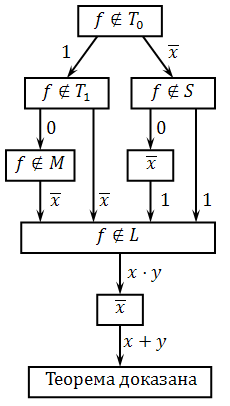
\includegraphics[scale=0.4]{images/post_sheme.png}
		\caption{Порядок перебора вариантов при доказательстве критерия Поста}
	\end{figure}
	
	Полное доказательство на \href{https://ru.wikipedia.org/wiki/%D0%9A%D1%80%D0%B8%D1%82%D0%B5%D1%80%D0%B8%D0%B9_%D0%9F%D0%BE%D1%81%D1%82%D0%B0}{Вики.}
\end{proof}


\subsection{Комбинаторные объекты. Коды Грея. Формула включения-исключения. Лемма Бернсайда и Теорема Пойа. Числа Стирлинга. Подсчёт деревьев. Метод производящих функций.}

\subsection{Детерминированные и недетерминированные конечные автоматы, их эквивалентность. Минимизация ДКА.}

\subsection{Математическая логика. Понятие доказательства. Правила вывода. Теоремы Гёделя.}

\subsection{Контекстно-свободные грамматики. Эффективные методы разбора: LL(k)-, LR(k)- и LALR-грамматики.}

\subsection{Комбинаторная теория сложности. Временная и емкостная сложность. Сложностные классы P, NP, PS. Сведение, NP-полные задачи.}

\subsection{Марковские цепи, Эргодические цепи, Регулярные цепи. Алгоритм Витерби.}

\subsection{Линейные структуры данных. Амортизационный анализ. Поисковые структуры данных. Запросы на отрезках. Персистентные структуры данных.}

\subsection{Графы. Обход графов. Поиск кратчайших путей. Задача о паросочетании, максимальном потоке и максимальном потоке минимальной стоимости.}

\subsection{Строки. Поиск строки в подстроке. Бор, алгоритм Ахо-Корасика. Суффиксные массивы и деревья.}

\subsection{Постановка задачи линейного программирования. Двойственность задачи ЛП.}

\subsection{Градиентные методы. Метод сопряжения градиентов. Минимизация квадратичных функций. Метод Ньютона.}

\newpage

\section{Программирование и вычислительная техника}

\subsection{Архитектура ЭВМ. Архитектура фон Неймана и гарвардская архитектура. Основные принципы и их альтернативы. Архитектура набора команд (ISA), CISC и RISC архитектуры.}

\subsubsection{Архитектура ЭВМ}
\textbf{Архитектура ЭВМ}~---~
это модель, устанавливающая принципы организации вычислительной системы, состав, 
порядок и взаимодействие основных частей ЭВМ, функциональные возможности, 
удобство эксплуатации, стоимость, надежность.

\subsubsection{Архитектура фон Неймана и гарвардская архитектура. Основные принципы и их альтернативы.}


\href{https://www.currentschoolnews.com/ru/%D0%BD%D0%BE%D0%B2%D0%BE%D1%81%D1%82%D0%B8-%D0%BE%D0%B1%D1%80%D0%B0%D0%B7%D0%BE%D0%B2%D0%B0%D0%BD%D0%B8%D1%8F/%D0%A0%D0%B0%D0%B7%D0%BD%D0%B8%D1%86%D0%B0-%D0%BC%D0%B5%D0%B6%D0%B4%D1%83-%D1%84%D0%BE%D0%BD-%D0%9D%D0%B5%D0%B9%D0%BC%D0%B0%D0%BD%D0%B0-%D0%B8-%D0%93%D0%B0%D1%80%D0%B2%D0%B0%D1%80%D0%B4%D1%81%D0%BA%D0%BE%D0%B9-%D0%B0%D1%80%D1%85%D0%B8%D1%82%D0%B5%D0%BA%D1%82%D1%83%D1%80%D1%8B/}{Подробнее тут}
\\

\textbf{Особенности архитектуры фон Неймана:}
\begin{enumerate}
	\item Архитектура фон Неймана - это теоретический проект, основанный на концепции компьютера с хранимой программой.
	\item Архитектура фон Неймана имеет только одну шину, которая используется как для извлечения инструкций, так и для передачи данных. Что еще более важно, операции должны быть запланированы, потому что они не могут быть выполнены одновременно.
	\item В архитектуре фон Неймана процессору потребовалось бы два тактовых цикла для выполнения инструкции.
	\item Архитектура фон Неймана обычно используется буквально на всех машинах, от настольных компьютеров, ноутбуков, высокопроизводительных компьютеров до рабочих станций.
\end{enumerate}

\textbf{Особенности Гарвардской aрхитектуры:}
\begin{enumerate}
	\item Гарвардская архитектура - это современная компьютерная архитектура, основанная на компьютерной модели ретранслятора Harvard Mark I.
	\item Гарвардская архитектура имеет отдельное пространство памяти для инструкций и данных, которое физически разделяет сигналы и код хранения и память данных, что, в свою очередь, позволяет получить доступ к каждой из систем памяти одновременно.
	\item В гарвардской архитектуре процессор может выполнить инструкцию за один цикл, если были установлены соответствующие планы конвейерной обработки.
	\item Гарвардская архитектура - это новая концепция, используемая специально в микроконтроллерах и цифровой обработке сигналов (DSP).
	\item Гарвардская архитектура - сложный вид архитектуры, поскольку в ней используются две шины для команд и данных, что делает разработку блока управления сравнительно более дорогой.
\end{enumerate}

\subsubsection{Архитектура набора команд (ISA), CISC и RISC архитектуры.}

\textbf{ISA}~---~архитектура набора команд, которая включает в себя систему и режимы адресации, спецификацию команд процессора, ригистры и типы данных, систему прерываний (для обработки ошибок во время вычисления)

Процессоры можно разделить по сложности набора команд:
\emph{CISC} (Complex Inst. Set Computer) vs \emph{RISC} (Reduced Inst. Set Computer).

\textbf{RISC}~---~Главная идея в поддержании небольшого набора простых и быстрых команд, под которые соптимизирован процессор. Предполагалось, что  сложные вызываются редко. Для этой архитектуры характерен фиксированная длина кодов команд, так как их проще декодировать и она не большая.

\textbf{CISC}~---~Тут у нас много команд для всяких сложных операций которые реализованы непосредственно на плате, что позволяет их ускорить, но это усложняет архитектуру и может мешать эффективной реализации простых команд, поэтому по количество операций в секунду такие процессоры проигрывают RICS. Так как количество команды большое, то характерна переменная длина кода (с Хаффман кодированием).

В современном мире по факту используется компромисс между этими подходами. Процессоры - CISC по спецификации, но внутри скорее RICS и конвертируют сложные в более простые + 0-level cache.

\subsection{Кратные, поверхностные и криволинейные интегралы. Формулы Грина, Стокса и Остроградского}


\subsubsection{Интеграль4ики}
\D{Пусть дана $f(x)$ -- функция действительной переменной. {\bf Неопределенным интегралом} функции $f(x)$, или ее первообразной, называется такая функция $F(x)$, производная которой равна $f(x)$, т.е. $F^{'}(x) = f(x)$. Обозначается $F(x) = \int f(x)dx$ }


\D{Кратным интегралом называют множество интегралов, взятых от $d > 1$, например  $$\underbrace{\int...\int f(x_1,...,x_d)dx_{1}...dx_{d}}_{d}$$}

Замечание -- кратный интеграл -- определенный интеграл, при его вычислении всегда получается число

\D{Криволинейный интеграл -- интеграл вычисляемый вдоль какой-либо прямой.
	
	Пусть $l$ -- пгладкая, без особых точек и пересечений кривая (может быть замкнутой), заданая параметрически $l: r(t)$, где $r$ -- радиус вектор, конец которого описывает кривую, а параметр $t$ направлен от начального значения $a$ к конечному значению $b$. Для интеграла второго рода направление, в котором движется параметр, определяет направление кривой $l$.
	
	Также есть скалярная или векторная функция , которая рассматривается вдоль кривой $l: f(r)$
	
	Еще есть разбиение отрезка параметризации, и разбиение кривой. Они соответствуют друг-другу (параметризация от параметра по факту сопостовляет точке из отрезка параметризации $[a, b]$ точку на прямой, и по разбиению параметризации разбивается кривая по соответствующим точкам, подробнее можно почитать на вики ссылку вставить не получилось:( )
	
	Интегральная сумма для интеграла {\bf первого рода} -- сумма вида $\sum\limits_{k=1}^{n} f(r(\xi_i))\cdot|l_k|$ где $|l_k|$ -- длина соответствующего отрезка, $\xi_i$ -- точка на соответствующем отрезке
	
	Интегральная сумма для интеграла {\bf первого рода} -- сумма вида $\sum\limits_{k=1}^{n} f(r(\xi_i))\cdot(r(t_k) = r(t_{k - 1})))$
	
	Собственно, криволинейный интеграл это интегральная сумма с $n$ устремленным в бесконечность
}

Похоже на обычный определенный интеграл, только тут мы вместо оси выравниваемся на кривую какую-то, и по факту считаем площидь криволинейного цилиндра между кривой в пространстве и ее проекцией (вроде бы, но это не точно)


\D{Пусть $\Phi$ -- гладкая, ограниченная полная поверхность. Пусть далее на $\Phi$ задана функция $f(M) = f(x, y, z)$. Рассмотрим разбиение $T$ этой поверхности на часть $\Phi_i (i=1, ..., n)$ кусочно-гладкими кривыми и на каждой такой части выберем произвольную точку $M_i(x_i, y_i, z_i)$. Вычислив значение функции в этой точке $f(M_i) = f(x_i, y_i, z_i)$ и, приняв за $\sigma_i$ площадь поверхность $\Phi_i$, рассмотрим сумму $$I\{\Phi_i, M_i\} = \sum_i f(M_i)\sigma_i$$. Тогда число I называется пределом сумм $i\{\Phi_i, M_i\}$ если $$\forall \epsilon > 0 \exists \delta > 0 \forall T: d(T) < \delta \forall \{M_i\} |I\{\Phi_i, M_i\} - I| < \epsilon$$
	Предел $I$ сумм $I\{\Phi_i, M_i\}$ при $d(T) \rightarrow 0$
	называется {\bf поверхностным интегралом первого рода} от функции $f(M)$ по поверхности $\Phi$ и обозначается $$I = \iint\limits_{\Phi} f(M)d\sigma$$} 

По сути -- берем поверхность в пространстве, а дальше как в криволинейном -- вместо отрезков оже куски пространства и т.д. получается магия какая-то.

Тут может быть полезно вспомнить про \href{https://mph.phys.spbu.ru/~budylin/meth/node15.html}{дифференциальные формы}

\subsubsection{Формула Грина}

\D{Пусть $C$ -- положительно ориентированная кусочно-гладкая замкнутая кривая на плоскости, а $D$ -- область, ограниченная кривой $C$. Если фунеции $P = P(x, y)$, $Q = Q(x, y)$ определены в области $D$ и имеют неприрывные частные производные $\frac{\partial P}{\partial y}, \frac{\partial Q}{\partial x}$, то $$\oint Pdx + Qdy = \iint\limits_{D}(\frac{\partial Q}{\partial x} - \frac{\partial P}{\partial y})dxdy$$}
{\bf Док-во и еще:} \href{https://ru.wikipedia.org/wiki/%D0%A2%D0%B5%D0%BE%D1%80%D0%B5%D0%BC%D0%B0_%D0%93%D1%80%D0%B8%D0%BD%D0%B0}{here}

\subsubsection{Формула Стокса}

\D{Пусть на ориентируемом многообразии $M$ размерности $n$ заданы положительно ориентированное ограниченное $p-$мерное подмногообразие $\sigma (1 \le p \le n)$ и дифференциальная форма $\omega$ степени $p - 1$ класса $C^1$. Тогда если граница подмногообразия $\partial \sigma$ положительно ориентированаб то $$\int\limits_{\sigma}d\omega = \int\limits_{\partial \sigma \omega}$$}

Грубо говоря взяли поверхность, и с помощью дифференциалов перешли к интегралу по границе поверхности, как-то так, но надо глубже разбираться потому что очень много определений которые надо помнить

\subsubsection{Формула Остроградского (Гаусс сосать)}

\D{Пусть теперь $\partial V$ -- кусочно-гладкая гипперповерхность $(p = n - 1)$, ограничивающая некоторую область $V$ в $n-$мерном пространстве. Тогда интеграл дивергенции (это оператор который отображает векторное поле на скалярное -- $div F = \lim\limits_{V \rightarrow 0} \frac{\Phi_F}{V}$, где $\Phi_F$ -- поток векторного поля $F$ через сферическую поверхность площадью $S$ ограничивающую объем $V$, хуита какая-то хочу объяснение на пальцах) поля по области равен потоку поля через границу области $\partial V$: $$\int\limits_{V} div F dV = \int\limits_{\partial V} F d \Sigma$$.
	
	В трехмерном пространстве $(n = 3)$ с координатами $\{x, y, z\}$ эквивалентнно $$\int\limits_{\partial V} F d \Sigma = \int\limits_{V}(\frac{\partial P}{\partial x} + \frac{\partial Q}{\partial y} + \frac{\partial R}{\partial z}) dV$$, или $$\iiint\limits_{\partial V} Pdydz + Qdzdx + Rdxdy = \iint\limits_{V} (\frac{\partial P}{\partial x} + \frac{\partial Q}{\partial y} + \frac{\partial R}{\partial z})dxdydz$$ }


Понятно что тут взяли и применили стокса на какой-то случай, но чет пиздец ребята)))

\subsection{С++. Процесс компиляции и линковки. .cpp, .h, .i, .o файлы.}
Понятно и подробно описано: 
\href{https://habr.com/ru/post/478124/}{https://habr.com/ru/post/478124/}

Кратко и структурировано: \href{https://server.179.ru/tasks/cpp/total/105.html}{https://server.179.ru/tasks/cpp/total/105.html}

\textbf{Компиляция}~---~трансляция программы, составленной на исходном языке высокого уровня, в эквивалентную программу на низкоуровневом языке, близком машинному коду (абсолютный код, объектный модуль, иногда на язык ассемблера). Входной информацией для компилятора (исходный код) является описание алгоритма или программа на объектно-ориентированном языке, а на выходе компилятора—эквивалентное описание алгоритма на машинно-ориентированном языке (объектный код).

\subsubsection{Заголовочные файлы (.h)}

%Целью заголовочных файлов является удобное хранение набора объявлений объектов для их последующего использования в других программах. 
В языках программирования Си и C++ заголовочные файлы~---~основной способ подключить к программе типы данных, структуры, прототипы функций, перечисляемые типы и макросы, используемые в другом модуле. По умолчанию используется расширение .h; иногда для заголовочных файлов языка C++ используют расширение .hpp.

Чтобы избежать повторного включения одного и того же кода, используются директивы \#ifndef, \#define, \#endif.

Заголовочный файл в общем случае может содержать любые конструкции языка программирования, но на практике исполняемый код (за исключением inline-функций в C++) в заголовочные файлы не помещают.

\subsection{С++. Жизненный цикл объектов в С++. RAII.}

\subsection{Линейные операторы в конечномерном пространстве и их матричное представление. Характеристический многочлен, собственные числа и собственные вектора линейного оператора. Сопряженные и самосопряженные операторы.}

\subsubsection{ Линейные операторы}

\D {Пусть $X$ и $Y$ -- линейные пространства над полем $F$. Отображение $\mathcal{A}: X \rightarrow Y$ называется линейным оператором, если $\forall x_1, x_2 \in X, \forall \lambda \in F$
	\begin{itemize}
		\item $\mathcal{A}(x_1 + x_2) = \mathcal{A}(x_1) + \mathcal{A}(x_2)$
		\item $\mathcal{A}(\lambda \cdot x_1) = \lambda \cdot \mathcal{A}(x_1)$
	\end{itemize}
	
	Линейный оператор $\mathcal{A}: X \rightarrow X$ называется автоморфизмом (или гомоморфизмом)
	
}

Операторы равны, если переводят элементы первого пространства в одинаковые элементы второго пространства.

\D{Пусть $\mathcal{A}: X \rightarrow Y$
	
	Пусть п.п. $X \leftrightarrow \{e_k\}_{k=1}^{n},\ \dim X = n$
	
	Пусть п.п. $Y \leftrightarrow \{h_k\}_{k=1}^{n},\ \dim Y = m$
	
	$\underset{{1\le k \le n}}{\mathcal{A}e_k} = \sum\limits_{i = 1}^{m} \alpha_k^i \cdot h_i \Rightarrow A = ||\alpha_k^i||,$ где $1 \le i \le m, 1 \le k \le m$
	
	$A = \begin{pmatrix}
		\alpha_1^1 & ... & \alpha_n^1\\
		\alpha_1^2 & ... & \alpha_n^2\\
		... & ... & ...\\
		\alpha_1^n & ... & \alpha_n^n\\
		
	\end{pmatrix}$
	
}

\subsubsection{Характеристический многочлен}

\D {Для данной матрицы $A$, $\chi(\lambda) = \det (A - \lambda E)$, где $E$ -- единичная матрица, является многочленом от $\lambda$, который называется {\bf характеристическим многочленом} матрицы $A$ (видимо можно отождествить матрицу с линейным оператором, тогда будет многочлен для оператора)}

Ценность характеристического многочлена в том, то собственные значения матрицы являются его корнями. Действительно, если уравнение $Av = \lambda v$ имеет ненулевое решение, то $(A - \lambda E)v = 0$, значит матрица $A - \lambda E$ вырождена и ее определитель $\det (A - \lambda E) = \chi(\lambda)$ равен 0

{\bf Свойства}

\begin{itemize}
	\item Для матрицы $n \times n$ характеристический многочлен имеет степень $n$
	\item Все корни характеристического многочлена матрицы являются ее собственными значениями
	\item Теорема Гамильтона-Кэли -- если $\chi(\lambda)$ -- характеристический многочлен матрицы $A$, то $\chi(A) = 0$
	\item Характеристические многочлены подобных матриц совпадают
	\item Характеристический многочлен обратной матрицы $\chi_{A^{-1}}(\lambda) = \frac{(-\lambda)^n}{\det A}\chi_A(1/\lambda)$
	\item Если $A$ и $B$ две матрицы $n \times n$, то $\chi_{AB} = \chi_{BA}$. В частности $tr(AB) = tr(BA), \det(AB) = \det (BA)$
	\item В более общем виде, если $A$ --матрица $m \times n$, а $B$ -- матрица $n \times m$, причем $m < n$, так что $AB$ и $BA$ --квадратные матрицы размеров $m$ и $n$ соответственно, то $\chi_{BA}(\lambda) = \lambda ^{n - m}\chi_{AB}(\lambda)$ 
\end{itemize}


\D{Пусть $L$ -- линейное пространство над полем $K$,
	
	$\mathcal{A}:L \rightarrow L$ -- линейный оператор
	
	{\bf Собственным вектором} линейного оператора $\mathcal{A}$ называется такой ненулевой вектор $x \in L$, что для некоторого $\lambda \in K: \mathcal{A}x = \lambda x$
	
	При этом $\lambda$ называют {\bf собственным числом} оператора $\mathcal{A}$
	
}

{\bf Свойства}

\begin{itemize}
	\item Собственные векторы, отвечающие различным собственным значениям, образуют ЛНЗ набор
	\item Еще какие-то леммы есть, подробнее см на \href{https://neerc.ifmo.ru/wiki/index.php?title=%D0%A1%D0%BE%D0%B1%D1%81%D1%82%D0%B2%D0%B5%D0%BD%D0%BD%D1%8B%D0%B5_%D0%B2%D0%B5%D0%BA%D1%82%D0%BE%D1%80%D1%8B_%D0%B8_%D1%81%D0%BE%D0%B1%D1%81%D1%82%D0%B2%D0%B5%D0%BD%D0%BD%D1%8B%D0%B5_%D0%B7%D0%BD%D0%B0%D1%87%D0%B5%D0%BD%D0%B8%D1%8F}{говне}
\end{itemize}

\subsubsection{Сопряженные и самосопряженные операторы}

\D{Пусть $E, L$ -- линейные пространства, а $E^*, L^*$ -- сопряженные линейные пространства (пространства линейных функционалов, определенных на $E$ и $L$). Тогда для любого линейного оператора $\mathcal{A}: E \rightarrow L$ и любого линейного функционала $g \in L^*$ определен линейный функционал $F \in E^*$ -- суперпозиция $g$ и $A: f(x) = g(A(x))$. Отображение $g \rightarrow f$ называется сопряженным линейным оператором и обозначается $\mathcal{A^*}: L^* \rightarrow E^*$. Если кратко, то $(\mathcal{A^*}g, x) = (g, \mathcal{A}x)$
	
	Если же $\mathcal{A^*} = \mathcal{A}$, то такой оператор называется самосопряженным, для него $(\mathcal{A}x, y) = (x, \mathcal{A}y)$
	
}

\subsection{Задача Коши для системы обыкновенных дифференциальных уравнений. Существование и единственность решения. Устойчивость.}

\href{https://ru.wikipedia.org/wiki/%D0%97%D0%B0%D0%B4%D0%B0%D1%87%D0%B0_%D0%9A%D0%BE%D1%88%D0%B8}{Вики}

\D{
	Обыкновенное дифференциальное уравнение (ОДУ) - дифференциальное уравнение для функции от одной переменной типа $F(x, y(x), y'(x), y''(x), \ldots, y^{(n)}(x)) = 0$. Нужно решить относительно функции $y$, т.е. найти такую функцию (или класс функций), что равенство верно в любой точке.
	
	Порядок ОДУ - максимальная производная. В примере выше - порядок $n$.
	
	Переменная при $y$ часто опускается.
}

В задаче Коши на неизвестную функцию накладывается \textbf{начальное условие}, т.е. значение в некоторой $x_0$.

Пример задачи Коши для ОДУ первого порядка:
\begin{align*}
	\begin{cases}
		y' = f(x, y)\\
		y(x_0) = y_0 
	\end{cases}
\end{align*}

Пример задачи Коши для многих функций ($y_1, y_2, \ldots, y_n$) только с первыми производными, иначе говоря \textit{Система $n$ ОДУ первого порядка}
\begin{align*}
	\begin{cases}
		y'_1 = f_1(x, y_1, y_2, \ldots, y_n)\\
		\vdots\\
		y'_n = f_n(x, y_1, y_2, \ldots, y_n)\\
		y_1(x_0) = y_{01}\\
		\vdots\\
		y_n(x_0) = y_{0n}
	\end{cases}
\end{align*}

Заметим, что здесь в правой части нет производных, т.е. эта система разрешена относительно производных (это называется нормальная форма). Еще, наверное, важно, что начальная точка одна для всех функций.

Конечно, можно сделать ОДУ порядка > 1, но будем честны, кого ебет.

\subsubsection{Существование и единственность решения}
Сформулируем для простейшей задачи Коши вида:
\begin{align*}
	\begin{cases}
		y' = f(x, y)\\
		y(x_0) = y_0 
	\end{cases}
\end{align*}

\href{http://twt.mpei.ac.ru/math/ode/odef/ODEf_04070000.html}{Формулировка.}

Основная мораль - что при определенных условиях на $f$ задача Коши имеет единственное решение в окрестности точки $x_0$. 

\subsubsection{Устойчивость}
Идея: если мы изменим начальное условие, изменится решение. Решение $\varphi(x)$ для начального условия $(x_0, y_{01})$ называется устойчивым по Ляпунову, если для любого другого решения $y$ с начальным условием $(x_0, y_{02})$ верно $\forall \varepsilon \exists \delta:\ \forall\ (x > x_0)\  (|y_{01} - y_{02}| < \delta \rightarrow |\varphi(x) - y(x)| < \varepsilon)$

\href{http://twt.mpei.ac.ru/math/ode/odef/ODEf_04100000.html}{Формулировка.} 



\subsection{Линейные обыкновенные дифференциальные уравнения и системы. Фундаментальная система решений. Метод вариации постоянных для решения неоднородных уравнений.}

\D{
	Обыкновенное дифференциальное уравнение (ОДУ) называется линейным, если оно имеет вид
	\begin{align*}
		y^{(n)} + a_{n-1}(x)y^{(n-1)} + \ldots + a_1(x)y' + a_0(x)y = f(x)
	\end{align*}
	Нужно решить относительно функции $y$, т.е. найти такую функцию (или класс функций), что равенство верно в любой точке.
	
	Мы решаем эту задачу для $x \in [a, b]$, и полагаем все $a_i$ и $f$ непрерывными на $[a, b]$.
}

Введем обозначения:
\begin{align*}
	Y = \begin{pmatrix}
		y_1\\
		\vdots\\
		y_n
	\end{pmatrix},\ 
	Y' = \begin{pmatrix}
		y_1'\\
		\vdots\\
		y_n'
	\end{pmatrix},\ 
	A(x) = \begin{pmatrix}
		a_{11}(x) & a_{12}(x) & \ldots & a_{1n}(x)\\
		a_{21}(x) & a_{22}(x) & \ldots & a_{2n}(x)\\
		\ldots & \ldots & \ldots & \ldots\\
		a_{n1}(x) & a_{n2}(x) & \ldots & a_{nn}(x)\\
	\end{pmatrix},\ 
	b(x) = \begin{pmatrix}
		b_1(x)\\
		\vdots\\
		b_n(x)\\
	\end{pmatrix}
\end{align*}

Тогда система дифференциальных уравнений в векторной (матричной) форме записывается в виде 
\begin{align*}
	Y' = A(x)Y + b(x)
\end{align*}

\T[Существование и единственность решения задачи Коши для линейной системы дифференциальных уравнений]{
	Если $A(x)$ и $b(x)$ непрерывны на отрезке $[a, b]$, то какова бы ни была начальная точка $(x_0, Y_0)$, задача Коши $Y' = A(x)Y + b(x), Y(x_0) = Y_0$, имеет единственное решение на $[a, b]$.  
}

\href{http://twt.mpei.ac.ru/math/ode/ODEsys/ODEsysup_08050000.html}{Формулировка.}

Принцип решения состоит в том, чтоб выражая и подставляя $y_i'$ как и в случае с числовыми системами, получить равенство, в которое входит только $y_i, y_i', \ldots y^{(n)}$, после чего решить ОДУ $n$-ого порядка. 
\href{https://math-it.petrsu.ru/users/semenova/DIFF_UR/Lections/Diff_UR_8.pdf}{Подробнее.} 

\subsubsection{Фундаментальная система решений}

\D{
	Если $b(x) = 0$, система называется однородной. Иначе - неоднородной.
}

\D{
	Фундаментальная система решений (ФСР) системы дифференциальных линейных однородных уравнений — максимальный (то есть содержащий наибольшее возможное число элементов) набор линейно независимых на $[a, b]$ решений этой системы
}

\D{
	Фундаментальная матрица - матрица, столбцы которой образуют ФСР
}

\T{Линейная однородная система уравнений имеет фундаментальную матрицу}

\T{
	Рассмотрим однородное уравнение $Y' = A(x)Y$. Если $W(x)$ - его фундаментальная матрица, то любое его решение $Y(x)$ представимо в виде $Y(x) = W(x)C$, где $C$ - произвольный постоянный вектор столбец.
}

Далее смотри \href{https://math-it.petrsu.ru/users/semenova/DIFF_UR/Lections/Diff_UR_8.pdf}{пособие} начиная со страницы 6, теоремы 5.

В пособии другие обозначения: 
\begin{align*}
	Y \rightarrow X\\
	A \rightarrow A\\
	x \rightarrow t\\
	b \rightarrow F(t)
\end{align*}

\subsubsection{Метод вариации постоянных для решения неоднородных уравнений}
Смотри \href{https://math-it.petrsu.ru/users/semenova/DIFF_UR/Lections/Diff_UR_8.pdf}{пособие} со страницы 7.

\subsection{Функциональное программирование. Чистые объекты. Функторы. Аппликативы. Монада. Взаимодействие с внешним миром.}

\subsubsection{Функциональное программирование. Чистые объекты.}
\textbf{Функциональное программирование}~---~парадигма программирования, в которой процесс вычисления трактуется как вычисление значений функций в математическом понимании последних (в отличие от функций как подпрограмм в процедурном программировании).

\textbf{Чистыми} называют функции, которые не имеют побочных эффектов ввода-вывода и памяти (они зависят только от своих параметров и возвращают только свой результат). Чистые функции обладают несколькими полезными свойствами, многие из которых можно использовать для оптимизации кода:
\begin{enumerate}
	\item если результат чистой функции не используется, её вызов может быть удалён без вреда для других выражений;
	\item результат вызова чистой функции может быть мемоизирован, то есть сохранён в таблице значений вместе с аргументами вызова;
	\item если нет никакой зависимости по данным между двумя чистыми функциями, то порядок их вычисления можно поменять или распараллелить (говоря иначе, вычисление чистых функций удовлетворяет принципам потокобезопасности);
	\item если весь язык не допускает побочных эффектов, то можно использовать любую политику вычисления. Это предоставляет свободу компилятору комбинировать и реорганизовывать вычисление выражений в программе (например, исключить древовидные структуры).
\end{enumerate}

\subsubsection{Функторы}

\href{https://habr.com/ru/post/183150/}{Объяснение на пальцах}

\href{http://cmc-msu-ai.github.io/haskell-course/lecture/2013/09/07/functors.html}{Подробнее про функторы}

\textbf{Функтором} называется класс типов, который декларирует единственный метод «fmap». Интуитивно, «fmap» применяет функцию a -> b к значению типа f a, чтобы получить значение типа f b. С другой стороны, можно рассматривать «fmap» как функцию высшего порядка, преобразующую «простую» функцию a -> b в «составную» функцию f a -> f b. Важно отметить, что структура значения типа f после применения «fmap» должна оставаться неизменной.

\begin{lstlisting}[language=Haskell]
	class Functor f where
	fmap :: (a -> b) -> f a -> f b
\end{lstlisting}

\subsubsection{Аппликативы.}
\href{http://cmc-msu-ai.github.io/haskell-course/lecture/2013/09/08/applicative-and-monad.html}{Подробнее тут}

Естественным продолжением класса Functor является класс \textbf{Applicative} (аппликативный функтор), определенный в модуле Control.Applicative:

\begin{lstlisting}[language=Haskell]
	class Functor f => Applicative f where
	pure  :: a -> f a
	(<*>) :: f (a -> b) -> f a -> f b
\end{lstlisting}

\textbf{Законы:}
\begin{enumerate}
	\item Помещение тождественной функции в «чистый» контекст и применение к аргументу в контексте не меняет ни значение, ни контекст.
	\begin{lstlisting}[language=Haskell]
		pure id <*> x == x
	\end{lstlisting}
	\item Применение чистой функции к чистому аргументу в контексте «по умолчанию» должно быть эквивалентно применению функции, а затем помещению результата в контекст.
	\begin{lstlisting}[language=Haskell]
		pure f <*> pure x == pure (f x)
	\end{lstlisting}
	\item При применении функции u с побочными эффектами к чистому аргументу y порядок вычисления функции и аргумента неважен.
	\begin{lstlisting}[language=Haskell]
		u <*> pure y == pure ($ y) <*> u
	\end{lstlisting}
	\item Некоторый аналог композиции для аппликативных функторов.
	\begin{lstlisting}[language=Haskell]
		u <*> (v <*> w) == pure (.) <*> u <*> v <*> w
	\end{lstlisting}
\end{enumerate} 

\subsubsection{Монады}
\href{http://cmc-msu-ai.github.io/haskell-course/lecture/2013/09/08/applicative-and-monad.html}{Подробнее тут}
\begin{lstlisting}[language=Haskell]
	class Monad m where
	return :: a -> m a
	(>>=) :: m a -> (a -> m b) -> mb
	(>>) :: m a -> m b -> m b
	m >> n = m >>= \_ -> n
	
	fail :: String -> m a
\end{lstlisting}

Функция return по типу очень напоминает функцию pure из класса Applicative. И, в действительности, return и есть pure, хоть и с не самым удачным названием (return в Haskell совсем не то же, что return в обычных императивных языках вроде C или Java). С математической точки зрения, любая монада является аппликативным функтором (но не наоборот). Но по историческим причинам,в описании класса это не указано.

Как следует из определения, операция ($>>$) является частным случаем операции ($>>=$)

Функция fail осталась в классе по историческим причинам, хотя никакого отношения к монадам реально не имеет.

\textbf{Законы:}
\begin{lstlisting}[language=Haskell]
	return a >>= k = k a
	m >>= return = m
	m >>= (\x -> k x >>= h) = (m >>= k) >>= h
	fmap f xs = xs >>= return . f = liftM f xs
\end{lstlisting}

\subsubsection{Взаимодействие с внешним миром.}
Взаимодействие с "внешним миром" (побочные эффекты вычислений) можно реализовать с помощью специальной монады IO.

Грубое приближение монады IO — это взятие пары с контекстом: "(a, RealWorld)". При операциях с монадой состояние RealWorld может меняться.

Есть операция return, погружающая объект в окружение IO («выпускающая во внешний мир»), а вот обратного преобразования нет.

\begin{lstlisting}[language=Haskell]
	putChar :: Char -> IO () 
\end{lstlisting}~---~берёт символ и возвращает новый «мир», в котором растворился (был напечатан в консоли) этот символ.

\begin{lstlisting}[language=Haskell]
	getChar :: IO Char
\end{lstlisting} --- мы можем получить символ из внешнего мира, но только внутри монады.

Достать его из монады мы не можем, но можем работать сним внутри IO с помощью $>>=$.

В процессе выполнения программы, содержащей IO, объекты типов IO a остаются временно невычисленными, как задумки.

Например, если мы где-то напишем putChar ' a' , то символ не будет тут же напечатан.

Вместо этого нужно дождаться, пока соберётся «главный» объект типа IO (), и уже при его вычислении все операции с внешним миром будут выполнены, причём в правильном порядке.

\subsection{Операционные системы. Процессы: вытесняющая и кооперативная многозадачность, планировщики, многопроцессорные машины.}

\textbf{Кооперативная многозадачность}.

Тип многозадачности, при котором фоновые задачи выполняются только во время простоя основного процесса и только в том случае, если на это получено разрешение основного процесса.

Кооперативную многозадачность можно назвать многозадачностью “второй ступени” поскольку она использует более передовые методы, чем простое переключение задач, реализованное многими известными программами (например, МS-DOS shell из МS-DOS 5.0 при простом переключении активная программа получает все процессорное время, а фоновые приложения полностью замораживаются). При кооперативной многозадачности приложение может захватить фактически столько процессорного времени, сколько оно считает нужным. Все приложения делят процессорное время, периодически передавая управление следующей задаче.

\textbf{ Вытесняющая многозадачность}.

Вид многозадачности, в котором операционная система сама передает управление от одной выполняемой программы другой. Распределение процессорного времени осуществляется планировщиком процессов. Этот вид многозадачности обеспечивает более быстрый отклик на действия пользователя.

Вытесняющая многозадачность~---~это вид многозадачности при котором планирование процессов основывается на абсолютных приоритетах. Процесс с меньшим приоритетом (например пользовательская программа) может быть вытеснен при его выполнении более приоритетным процессом (например системной или диагностической программой). Иногда этот вид многозадачности называют приоритетным.

Каждая работающая программа имеет свое защищенное адресное пространство. Многопоточное выполнение отдельных задач позволяет при задержке в выполнении одного потока не останавливать задачу полностью, а работать со следующим потоком.

\textbf{Планировщик.}

\href{https://habr.com/ru/post/154609/}{Подробнее тут}

Планировщик~---~часть операционной системы, которая отвечает за (псевдо)параллельное выполнения задач, потоков, процессов. Планировщик выделяет потокам процессорное время, память, стек и прочие ресурсы. Планировщик может принудительно забирать управление у потока (например по таймеру или при появлении потока с большим приоритетом), либо просто ожидать пока поток сам явно(вызовом некой системной процедуры) или неявно(по завершении) отдаст управление планировщику.
Первый вариант работы планировщика называется реальным или вытесняющим(preemptive), второй, соответственно, не вытесняющим (non-preemptive).

\textbf{Многопроцессорные машины.}

\href{https://docstore.mik.ua/skbd/glava_10.htm}{Подробнее тут}

\href{https://ru.wikipedia.org/wiki/%D0%9C%D0%BD%D0%BE%D0%B3%D0%BE%D0%BF%D1%80%D0%BE%D1%86%D0%B5%D1%81%D1%81%D0%BE%D1%80%D0%BD%D0%BE%D1%81%D1%82%D1%8C}{В Википедии тоже хорошо написано}

Любая вычислительная система (будь то супер-ЭВМ или персональный компьютер) достигает своей наивысшей производительности благодаря использованию высокоскоростных элементов и параллельному выполнению большого числа операций. Именно возможность параллельной работы различных устройств системы (работы с перекрытием) является основой ускорения основных операций. 

Параллельные ЭВМ часто подразделяются по классификации Флинна на машины типа SIMD (Single Instruction Multiple Data - с одним потоком команд при множественном потоке данных) и MIMD (Multiple Instruction Multiple Data - с множественным потоком команд при множественном потоке данных). Как и любая другая, приведенная выше классификация несовершенна: существуют машины прямо в нее не попадающие, имеются также важные признаки, которые в этой классификации не учтены. В частности, к машинам типа SIMD часто относят векторные процессоры, хотя их высокая производительность зависит от другой формы параллелизма - конвейерной организации машины. Многопроцессорные векторные системы, типа Cray Y-MP, состоят из нескольких векторных процессоров и поэтому могут быть названы MSIMD (Multiple SIMD).

\subsection{Операционные системы. Виртуальная память: MMU, TLB, таблицы страниц, аллокаторы и менеджеры виртуальной памяти.}

\subsubsection{Виртуальная память: MMU, TLB.}

\href{https://habr.com/ru/post/211150/}{Подробнее тут}

Блок управления памятью или устройство управления памятью memory management unit, MMU)~---~компонент аппаратного обеспечения компьютера, отвечающий за управление доступом к памяти, запрашиваемым центральным процессором.

Его функции заключаются в трансляции адресов виртуальной памяти в адреса физической памяти (то есть управление виртуальной памятью), защите памяти, управлении кэш-памятью, арбитражем шины и, в более простых компьютерных архитектурах (особенно 8-битных), переключением блоков памяти. 

Принцип работы современных MMU основан на разделении виртуального адресного пространства (одномерного массива адресов, используемых центральным процессором) на участки одинакового, как правило, несколько килобайт, хотя, возможно, и существенно большего, размера, равного степени 2, называемые страницами. Младшие n бит адреса (смещение внутри страницы) остаются неизменными. Старшие биты адреса представляют собой номер (виртуальной) страницы. MMU обычно преобразует номера виртуальных страниц в номера физических страниц, используя буфер ассоциативной трансляции (Translation Lookaside Buffer, TLB).

Если преобразование при помощи TLB невозможно, включается более медленный механизм преобразования, основанный на специфическом аппаратном обеспечении или на программных системных структурах. Данные в этих структурах, как правило, называются элементами таблицы страниц (page table entries (PTE)), а сами структуры — таблицами страниц (англ. page table (PT)). Конкатенация номера физической страницы со смещением внутри страницы даёт физический адрес.

Элементы PTE или TLB могут также содержать дополнительную информацию: бит признака записи в страницу ( dirty bit), время последнего доступа к странице (accessed bit), какие процессы (пользовательские (user mode) или системные (supervisor mode)) могут читать или записывать данные в страницу, необходимо ли кэшировать страницу.

\subsubsection{Таблицы страниц.}

\href{https://ru.wikipedia.org/wiki/%D0%A2%D0%B0%D0%B1%D0%BB%D0%B8%D1%86%D0%B0_%D1%81%D1%82%D1%80%D0%B0%D0%BD%D0%B8%D1%86}{Википедия}

Таблица страниц~---~это структура данных, используемая системой виртуальной памяти в операционной системе компьютера для хранения сопоставления между виртуальным адресом и физическим адресом. Виртуальные адреса используются выполняющимся процессом, в то время как физические адреса используются аппаратным обеспечением, или, более конкретно, подсистемой ОЗУ. Таблица страниц является ключевым компонентом преобразования виртуальных адресов, который необходим для доступа к данным в памяти.

\subsubsection{Аллокаторы.}

\href{https://habr.com/ru/post/505632/}{Подробнее тут}

Аллокатор или распределитель памяти в языке программирования C++ ~---~ специализированный класс, реализующий и инкапсулирующий малозначимые (с прикладной точки зрения) детали распределения и освобождения ресурсов компьютерной памяти.

Концептуально выделяется пять основных операции, которые можно осуществить над аллокатором:
\begin{enumerate}
	\item \emph{create}~---~создает аллокатор и отдает ему в распоряжение некоторый объем памяти;
	\item \emph{allocate}~---~выделяет блок определенного размера из области памяти, которым распоряжается аллокатор;
	\item \emph{deallocate}~---~освобождает определенный блок;
	\item \emph{free}~---~освобождает все выделенные блоки из памяти аллокатора (память, выделенная аллокатору, не освобождается);
	\item \emph{destroy}~---~уничтожает аллокатор с последующим освобождением памяти, выделенной аллокатору.
\end{enumerate}

\subsubsection{Менеджеры виртуальной памяти.}

Менеджер виртуальной памяти (далее просто «менеджер памяти») ~---~ часть операционной системы, благодаря которой можно адресовать память большую, чем объем физической памяти (ОЗУ).

Благодаря виртуальной памяти можно запускать множество ресурсоёмких приложений, требующих большого объёма ОЗУ. Максимальный объём виртуальной памяти, который можно получить, используя 24-битную адресацию, — 16 мегабайт. С помощью 32-битной адресации можно адресовать до 4 ГБ виртуальной памяти. А 64-битная адресация позволяет работать уже с 16 эксабайтами памяти.

Применение механизма виртуальной памяти позволяет:

\begin{enumerate}
	\item упростить адресацию памяти клиентским программным обеспечением;
	\item рационально управлять оперативной памятью компьютера (хранить в ней только активно используемые области памяти);
	\item изолировать процессы друг от друга (процесс полагает, что монопольно владеет всей памятью).
\end{enumerate}


\subsection{Вероятностные неравенства Йенсена, Маркова и Чебышёва. Правило трёх сигм. Закон больших чисел}

\subsubsection{Неравенство Йенсена}

\D {Пусть $(\Omega, \mathcal{F}, \mathbb{P})$ -- вероятностное пространство, и $X: \Omega \rightarrow \mathbb{R}$ -- определенная на нем случайная величина. Пусть также $\phi: \mathbb{R} \rightarrow \mathbb{R}$ -- выпуклая (вниз) борелевская функция. Тогда если $X, \phi(X) \in L^1 (\Omega, \mathcal{F}, \mathbb{P})$, то
	$$\phi(EX) \le E(\phi(X))$$. Также можно добавить условность}

\subsubsection{Неравенство Маркова}

\D {Пусть неотрицательная случайная величина $X: \Omega \rightarrow \mathbb{R}^{+}$ определена на вероятностном пространстве, и ее матожидание конечно. Тогда 
	
	$\mathbb{P}(X \ge a) \le \frac{EX}{a}$}

{\bf Док-во:}

Пусть неотрицательная лучайная величина $X$ имеет плотность распределения $p(x)$, тогда для $a > 0$

$EX = \int\limits_{0}^{\infty} xp(x)dx \ge \int\limits_{a}^{\infty}xp(x)dx \ge \int\limits_{a}^{\infty}ap(x)dx = a \mathbb{P}(X \ge a)$


\subsubsection{Неравенство Чебышева}

\D {Пусть случайная величина $X$ определена на вероятностном пространстве, а ее матожидание $\mu$ и дисперсия $\sigma^2$ конечны. Тогда
	
	$P(|X - \mu| \ge a) \le \frac{\sigma^2}{a^2}, a > 0$
	
	Если $a = k\sigma$, где $\sigma$ -- стандартное отклонение, $k > 0$, то получаем
	
	$P(|X - \mu| >\ge k\sigma) \le \frac{1}{k^2}$
}


\subsubsection{Правило трех сигм}

Если случайная величина распределена нормально, то абсолютная величина ее отклонения от матожидания не превосходит утроенного среднего квадратического отклонения

$P(|X - \mu| \ge 3 \sigma) \le \frac{1}{9}$


\subsubsection{Закон больших чисел}

\D {Рассмотрим последовательность независимых в совокупности случайных величин $X_1, X_2, ...$ интегрируемых по Лебегу, которые имеют одинаковые распределения, следовательно, и одинаковые матожидания. Обозначим через $\overline{X}_n$ среднее арифметическое рассматриваемых случайных величин. Оно сходится к матожиданию}

{\bf Слабый закон}

Сходится по вероятности к матожиданию 

$\overline{X}_n \rightarrow \mu$ при $n \rightarrow 0$

\subsection{Множества и операции над ними. Булевы функции, КНФ, ДНФ. Базисы, теорема Поста.}

\subsubsection{Множества и операции над ними}

\subsubsection{Булевы функции, КНФ, ДНФ}
\T{В ДНФ можно выразить любую функцию}
\begin{proof}
	Рассмотрим строчки таблицы истинности с 1, для каждой напишем клоз из $n$ лиетралов, который выполняет ровно эту строчку.
	
	Википедия чета пишет про то, что тождественный 0 нельзя представить. Вообще можно, если можно писать $x \wedge \neg x$
\end{proof}

\T{В КНФ можно выразить любую булеву функцию}
\begin{proof}
	Построим ДНФ к отрицанию, повесим отрицание, по де-Моргану получим КНФ 
\end{proof}

\subsubsection{Базисы, теорема Поста}

Хуеста, блять, как же я затрахался. 

Булевы функции можно получать из других при помощи композиции. Возникает естественный вопрос, какими наборами функций можно выразить любую функцию.

\D{
	Стрелка Пирса: $x \uparrow y = \neg (x \vee y)$ 
}
\T{
	Стрелка Пирса - полный базис
}
\begin{proof}
	Получим конъюнкцию, дизъюнкцию и отрицание
	\begin{enumerate}
		\item $\neg x = x \uparrow x$
		\item $x \vee y = \neg (x \uparrow y)$
		\item $x \wedge y = \neq (\neg x \vee \neq y)$
	\end{enumerate}
\end{proof}

Вот Пост придумал критерий, как по набору функций понять, является ли он полным.

\textit{Замыкание класса функций} - это множество всех их возможных композиций.

Мы предъявляем 5 классов функций:
\begin{align*}
	T_0 = \{f \mid f(\overline{0}) = 0\}\\
	T_1 = \{f \mid f(\overline{1}) = 1\}\\
	M = \{f \mid \forall \alpha, \beta \in \mathbb{B}^n\ (\alpha \geq \beta) \rightarrow f(\alpha) \geq f(\beta)\}\\
	S = \{f \mid \forall \alpha \in \mathbb{B}^n f(\alpha) = \overline{f(\overline{\alpha})}\}\\
	L = \{f \mid f(x_1, x_2, \ldots x_n) = \alpha_0 \oplus \alpha_1x_1 \oplus \ldots \oplus \alpha_nx_n\}
\end{align*}

\T[Критерий поста]{
	Множество функций $F$ полно тогда и только тогда, когда в нем (его замыкании относительно композиций) есть функция, не принадлежащая ни одному из классов выше.
}

\begin{proof}
	Понятно, что если замыкание $F$ содержится в одном из классов, то $F$ не полно, т.к. ни один из классов не совпадает со множеством всех функций.
	
	В другую сторону докажем, что в $F$ можно реализовать конъюнкцию дизъюнкцию и отрицание. 
	
	\begin{figure}[H]
		\centering
		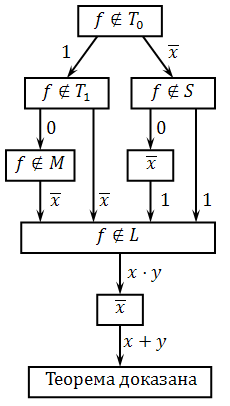
\includegraphics[scale=0.4]{images/post_sheme.png}
		\caption{Порядок перебора вариантов при доказательстве критерия Поста}
	\end{figure}
	
	Полное доказательство на \href{https://ru.wikipedia.org/wiki/%D0%9A%D1%80%D0%B8%D1%82%D0%B5%D1%80%D0%B8%D0%B9_%D0%9F%D0%BE%D1%81%D1%82%D0%B0}{Вики.}
\end{proof}


\subsection{Комбинаторные объекты. Коды Грея. Формула включения-исключения. Лемма Бернсайда и Теорема Пойа. Числа Стирлинга. Подсчёт деревьев. Метод производящих функций.}

\subsubsection{Коды Грея}
Код Грея - код для элементов упорядоченного множества (например, чисел от 1 до $n$), такой что расстояние Хэмминга между кодами соседних элементов = 1.
\begin{figure}[H]
	\centering
	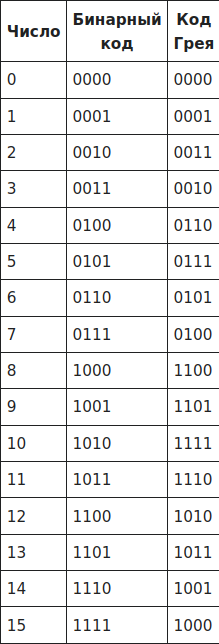
\includegraphics[scale=0.4]{images/grey.png}
\end{figure}

Коды Грея легко получаются из двоичных чисел путём побитовой операции «Исключающее ИЛИ» с тем же числом, сдвинутым вправо на один бит и в котором старший разряд заполняется нулём. Следовательно, $i$-й бит кода Грея $G_i$ выражается через биты двоичного кода $B_i$ следующим образом:
\begin{align*}
G_i = B_i \oplus B_i + 1
\end{align*}

где $\oplus$ — операция «исключающее ИЛИ»; биты нумеруются справа налево, начиная с младшего. 

Декодинг происходит по формуле 
\begin{align*}
	B_i = B_{i + 1} \oplus G_i
\end{align*}

Код Грея назван «рефлексивным» (отражённым) из-за того, что первая половина значений при изменении порядка эквивалентна второй половине, за исключением старшего бита. Старший бит просто инвертируется. При делении каждой новой половины пополам это свойство сохраняется.

Код Грея используется в тех случаях, когда мы медленно считываем значения, а они меняются. Представим себе, что код (обычный двоичный) перескакивает $3\rightarrow4$, или $011_2 \rightarrow 100_2$. Если из-за несовершенства считывателя мы прочитаем первый бит от $011$, а остальные два — от $100$, мы получим $000_2=0$ — число, далёкое от реальных значений. В коде Грея никаких посторонних значений не будет: перескок будет в одном разряде, $010_G \rightarrow 110_G$, и мы считаем либо старое $010_G=3$, либо новое $110_G=4$. 

\subsubsection{Формула включения-исключения}

\T{
	Пусть $A = \bigcup\limits_{i = 1}^nA_i$, тогда по формуле включения-исключения:
	\begin{align*}
		|A| = \sum\limits_{I \in 2^n - 1}(-1)^{|I| + 1}|\bigcap_{j\in I}A_j|
	\end{align*}

	где $N = \{1, \ldots n\}$, $2^N - 1$ - множество всех непустых подмножеств $N$. 
}
\begin{proof}
	\href{https://neerc.ifmo.ru/wiki/index.php?title=%D0%A4%D0%BE%D1%80%D0%BC%D1%83%D0%BB%D0%B0_%D0%B2%D0%BA%D0%BB%D1%8E%D1%87%D0%B5%D0%BD%D0%B8%D1%8F-%D0%B8%D1%81%D0%BA%D0%BB%D1%8E%D1%87%D0%B5%D0%BD%D0%B8%D1%8F}{Доказательство}.
\end{proof}

Формулу включений исключений можно интерпретировать в вероятностном смысле, нужно лишь заменить множества на события, а мощности на вероятности. 

\subsubsection{Лемма Бернсайда}
Я чета в ахуе немного, это из теории групп. Про орбиты. 

\D{
	Говорят, что группа $G$ действует на множестве $M$ слева, если задано отображение $G \times M \rightarrow M$, такое что
	\begin{enumerate}
		\item $g(hm) = (gh)m$ для всех $g, h \in G, m \in M$
		\item $em = m$, где $e$ - нейтральный элемент $G$
	\end{enumerate}
}

\D{
	Подмножество
	\begin{align*}
		Gm = \{gm \mid g \in G\} \subset M
	\end{align*}

	Называется орбитой элемента $m$
}

\T[Лемма Бернсайда]{
	Пусть $G$ — конечная группа, действующая на множестве $X$. Тогда число орбит действия равно среднему количеству точек, фиксированных точек в $X$ элементами $G$.
	
	Точнее, для любого элемента $g \in G$ будем обозначать через $X^g$ множество элементов $X$, оставляемых на месте $g$, то есть
	\begin{align*}
		X^g = \{x \in X \mid gx = x\}
	\end{align*} 

	Тогда
	\begin{align*}
		|X/G| = \frac{1}{|G|}\sum\limits_{g \in G}|X^g|
	\end{align*}
	
	где $|X/G|$ - обозначает число орбит действия.
}
\begin{proof}
	\href{https://neerc.ifmo.ru/wiki/index.php?title=%D0%9B%D0%B5%D0%BC%D0%BC%D0%B0_%D0%91%D1%91%D1%80%D0%BD%D1%81%D0%B0%D0%B9%D0%B4%D0%B0_%D0%B8_%D0%A2%D0%B5%D0%BE%D1%80%D0%B5%D0%BC%D0%B0_%D0%9F%D0%BE%D0%B9%D0%B0#.D0.A2.D0.B5.D0.BE.D1.80.D0.B5.D0.BC.D0.B0_.D0.9F.D0.BE.D0.B9.D0.B0}{Доказательство}.
\end{proof}


\subsubsection{Теорема Пойа}
\href{https://e-maxx.ru/algo/burnside_polya}{Тут} максимально просто написано и про Пойа и про Бернсайда.

\subsubsection{Числа Стирлинга}
\begin{itemize}
	\item \textit{Первого рода.} Количество перестановок из $n$ элементов с $k$ циклами.
	
	Можно посчитать рекурсивно:
	\begin{align*}
		c(n, k) = c(n - 1, k - 1) + (n - 1)\cdot c(n - 1, k)
	\end{align*} 
	\item \textit{Второго рода.} Количество неупорядоченных разбиений $n$-элементного множества на $k$ непустых подмножеств.
	
	Можно посчитать рекурсивно:
	\begin{align*}
		S(n, k) = S(n - 1, k - 1) + k\cdot S(n - 1, k)
	\end{align*}
	
	Есть явная формула:
	\begin{align*}
		S(n, k) = \frac{1}{k!}\sum\limits(-1)^{k + j}{k \choose j}j^n
	\end{align*}
\end{itemize}

\subsubsection{Подсчет деревьев}
\D{
	$n$-ое число Каталана:
	\begin{align*}
		C_n = \frac{1}{n + 1}\binom{2n}{n}
	\end{align*}

	Числа Каталана - удовлетворяют рекуррентному соотношению
	\begin{align*}
		C_0 = 1\\
		C_n = \sum\limits_{i =0}^{n - 1}C_iC_{n - 1 - i}
	\end{align*}
	Например, это количество правильных скобочных последовательностей длины $2n$.
}

Более подробно на \href{https://ru.wikipedia.org/wiki/%D0%A7%D0%B8%D1%81%D0%BB%D0%B0_%D0%9A%D0%B0%D1%82%D0%B0%D0%BB%D0%B0%D0%BD%D0%B0}{Вики}.

\T{
	Количество неизоморфных упорядоченных бинарных деревьев с корнем и $n + 1$ листьями = $n$-ому числу Каталана. 
	
	Здесь \textit{упорядоченные} означает, что ребра, выходящие из каждой вершины, упорядочены.
}

\D{
	Помеченное дерево c $n$ вершинами - дерево c $n$ вершинами, вершинам которого взаимно однозначно соответствуют числа от 1 до $n$.
}

\T[Кэли]{
	Число помеченных деревьев с $n$ вершинами равняется $n^{n - 2}$.
}
\begin{proof}
	Доказательство и еще много всего интересного смотри \href{https://neerc.ifmo.ru/wiki/index.php?title=%D0%9F%D0%BE%D0%B4%D1%81%D1%87%D0%B5%D1%82_%D0%B4%D0%B5%D1%80%D0%B5%D0%B2%D1%8C%D0%B5%D0%B2}{тут}. 
\end{proof}

\subsubsection{Метод производящих функций}
Вот \href{https://neerc.ifmo.ru/wiki/index.php?title=%D0%9F%D1%80%D0%BE%D0%B8%D0%B7%D0%B2%D0%BE%D0%B4%D1%8F%D1%89%D0%B0%D1%8F_%D1%84%D1%83%D0%BD%D0%BA%D1%86%D0%B8%D1%8F}{отсюда} можно прочитать определение и пример для решения рекуррент


\subsection{Параллельное программирование. Консенсусное число. Стек Трайбера. Очередь Майкла-Скотта.}

\href{https://www.babichev.org/tpmtp/Lecture09.pdf}{Про консенсус}.
\D{
	Задача консенсуса: есть $N$ потоков, нужно чтоб они все пришли к согласию по поводу какого-то одного значения.
}

\D{
	Любой последовательный объект можно реализовать без ожидания (wait-free) для N потоков используя консенсусный протокол для N потоков.
	
	Такое построение называется универсальная конструкция
}	

\href{https://neerc.ifmo.ru/wiki/index.php?title=%D0%A1%D1%82%D0%B5%D0%BA_%D0%A2%D1%80%D0%B0%D0%B9%D0%B1%D0%B5%D1%80%D0%B0}{Стек Трайбера}

\href{https://neerc.ifmo.ru/wiki/index.php?title=%D0%9E%D1%87%D0%B5%D1%80%D0%B5%D0%B4%D1%8C_%D0%9C%D0%B0%D0%B9%D0%BA%D0%BB%D0%B0_%D0%B8_%D0%A1%D0%BA%D0%BE%D1%82%D1%82%D0%B0}{Очередь Майкла-Скотта}.

\subsection{Математическая логика. Понятие доказательства. Правила вывода. Теоремы Гёделя.}

\D{
	Формальная дедуктивная теория состоит из
	\begin{itemize}
		\item Алфавита
		\item Правила образований формул (чисто синтаксически)
		\item Аксиом (подмножества формул)
		\item Правил вывода (способов получать из одних формул другие)
	\end{itemize}
}

Пример - \href{https://ru.wikipedia.org/wiki/%D0%9B%D0%BE%D0%B3%D0%B8%D0%BA%D0%B0_%D0%B2%D1%8B%D1%81%D0%BA%D0%B0%D0%B7%D1%8B%D0%B2%D0%B0%D0%BD%D0%B8%D0%B9#%D0%90%D0%BA%D1%81%D0%B8%D0%BE%D0%BC%D1%8B_%D0%B8_%D0%BF%D1%80%D0%B0%D0%B2%D0%B8%D0%BB%D0%B0_%D0%B2%D1%8B%D0%B2%D0%BE%D0%B4%D0%B0_%D1%84%D0%BE%D1%80%D0%BC%D0%B0%D0%BB%D1%8C%D0%BD%D0%BE%D0%B9_%D1%81%D0%B8%D1%81%D1%82%D0%B5%D0%BC%D1%8B_%D0%BB%D0%BE%D0%B3%D0%B8%D0%BA%D0%B8_%D0%B2%D1%8B%D1%81%D0%BA%D0%B0%D0%B7%D1%8B%D0%B2%D0%B0%D0%BD%D0%B8%D0%B9}{логика исчисления высказываний}.

Самым распространенным (а в случае с логикой исчисления высказываний единственным) правилом вывода является Modus ponens:
\begin{align*}
	\dfrac{A\ A \rightarrow B}{B}
\end{align*}

\D{
Формула $F$ называется выводимой из множества формул $\Gamma$, если ее можно получить из $\Gamma$ при помощи правил вывода.
}

\D{
Формула $F$ называется доказуемой, если ее можно вывести из аксиом. 
}

Более подробно про вывод \href{http://fkn.univer.omsk.su/kursi/disc/prlogic.htm#2.9}{тут}. (или можете у меня (Антона) спросить, я вроде чета понимаю про это).

У логик есть два важных свойства:
\begin{itemize}
	\item \textbf{Непротиворечивость.} Теория, в которой множество теорем покрывает всё множество формул (все формулы являются теоремами, «истинными высказываниями»), называется противоречивой. В противном случае теория называется непротиворечивой.
	\item \textbf{Полнота.} Теория называется полной, если в ней для любого предложения $F$ выводимо либо само $F$, либо его отрицание $\neg F$. В противном случае, теория содержит недоказуемые утверждения (утверждения, которые нельзя ни доказать, ни опровергнуть средствами самой теории), и называется неполной. 
\end{itemize}

\D{
	Арифметика - система аксиом Пеано для натуральных чисел.
}

Вики про \href{https://ru.wikipedia.org/wiki/%D0%90%D0%BA%D1%81%D0%B8%D0%BE%D0%BC%D1%8B_%D0%9F%D0%B5%D0%B0%D0%BD%D0%BE}{акисомы Пеано}.

\T[Первая теорема Гёделя (О неполноте)]{
	Если арифметика непротиворечива, то она не полна. 
	
	Иначе говоря, если с помощью аксиом Пеано не выводятся вообще все утверждения о натуральных числах, то существует утверждение, которое нельзя ни доказать, ни опровергнуть. 
}
\begin{proof}
	Если вкратце, то в арифметике можно закодировать высказывание $A$ "это высказывание не выводимо в арифметике". Понятно, что, как и с парадоксом лжеца, это высказывание нельзя ни доказать (предъявить вывод), ни опровергнуть (предъявить вывод отрицания).
	
	На \href{https://ru.wikipedia.org/wiki/%D0%A2%D0%B5%D0%BE%D1%80%D0%B5%D0%BC%D0%B0_%D0%93%D1%91%D0%B4%D0%B5%D0%BB%D1%8F_%D0%BE_%D0%BD%D0%B5%D0%BF%D0%BE%D0%BB%D0%BD%D0%BE%D1%82%D0%B5}{вики} есть набросок доказательства.
\end{proof}

\T[Вторая теорема Гёделя]{
	В формальной арифметике также можно закодировать формулу $G$, говорящую "формальная арифметика непротиворечива". И если арифметика непротиворечива, то эту формулу нельзя вывести.
	
	Другими словами, изнутри теории нельзя доказать ее собственную непротиворечивость. 
	
	Эта формула является конкретным примером к первой теореме.
}
\begin{proof}
	Назовем формулу, говорящую "арифметика непротиворечива" $Con$ (эту формулу вполне можно выписать на языке арифметики). Вспомним формулу $A$ из первой теоремы, говорящую "$A$ не выводима в арифметике".
	
	Тогда первая теорема Гёделя выглядит так:
	\begin{align*}
		Con \rightarrow A
	\end{align*}
	
	Мы знаем, что это высказывание верно (и доказательство может быть превращено в формальный арифметический вывод, т.е. оно выводимо в арифметике). 
	
	Теперь, если $Con$ выводима, то мы сможем ее вывести, а затем, применив Modus ponens к ней и первой теореме Гёделя, выведем $A$, но $A$ не выводима, если арифметика непротиворечива. Таким образом, $Con$ не выводима.
\end{proof}

\subsection{Компьютерные сети. DHCP, DNS, NAT. Интернет-протоколы.}

\subsection{Комбинаторная теория сложности. Временная и емкостная сложность. Сложностные классы P, NP, PS. Сведение, NP-полные задачи.}

\T{
	$P = NP$
}

\href{https://ru.wikipedia.org/wiki/%D0%A1%D0%B2%D0%B5%D0%B4%D0%B5%D0%BD%D0%B8%D0%B5_(%D1%82%D0%B5%D0%BE%D1%80%D0%B8%D1%8F_%D1%81%D0%BB%D0%BE%D0%B6%D0%BD%D0%BE%D1%81%D1%82%D0%B8_%D0%B2%D1%8B%D1%87%D0%B8%D1%81%D0%BB%D0%B5%D0%BD%D0%B8%D0%B9)}{Сведение}

\subsection{Базы данных. Реализация реляционных СУБД. Индексы, применение индексов. Транзакции, свойства транзакций. Блокировки, типы блокировок.}

\href{https://www.dropbox.com/sh/4st5b16mvdf8gkj/AADo-NrUSL5vJLWDfeAFWwy1a/Programming/13%20%D0%A0%D0%B5%D0%BB%D1%8F%D1%86%D0%B8%D0%BE%D0%BD%D0%BD%D1%8B%D0%B5%20%D0%A1%D0%A3%D0%91%D0%94.pdf?dl=0}{dropbox}

\subsection{Шаблоны проектирования, их применение. Классификация шаблонов проектирования. Примеры шаблонов проектирования.}

\href{https://www.dropbox.com/sh/4st5b16mvdf8gkj/AACWB4gDVx73cjp5xudo1nGma/Programming/18%20%D0%A8%D0%B0%D0%B1%D0%BB%D0%BE%D0%BD%D1%8B%20%D0%BF%D1%80%D0%BE%D0%B5%D0%BA%D1%82%D0%B8%D1%80%D0%BE%D0%B2%D0%B0%D0%BD%D0%B8%D1%8F.pdf?dl=0}{dropbox}

\subsection{Теория кодирования. Блоковые коды и их параметры. Критерии декодирования и метрики. Границы Хемминга и Варшамова-Гилберта.}

\subsection{Теория кодирования. Линейные коды. Границы Синглтона, ВаршамоваГилберта и Грайсмера. Вероятность ошибки декодирования и необнаружения ошибки.}

\subsection{Машинное обучение. Понятие машинного обучения в искусственном интеллекте. Классификация задач машинного обучения, их примеры и особенности.}

\subsection{Машинное обучение. Многослойная нейронная сеть и алгоритм обратного распространения ошибок. Методы инициализации и методы оптимизации в нейронных сетях. Архитектуры сетей, их применение}

\end{document}
